\documentclass{mythesis}


% PGFPLOTS STUFF
\usepackage{pgfplots}
\pgfplotsset{compat=1.11}
\usepgfplotslibrary{external}
\tikzexternalize
\pgfplotsset{every axis/.append style={no markers}}
\pgfplotsset{every axis legend/.append style={
    at={(1.02,1)},
    anchor=north west
}}


\DeclareDocumentCommand{\myincludegraphics}{om}{
    \begin{tikzpicture}
	\node[draw=black!30,inner sep=0] {
	    \includegraphics[#1]{#2}
	};
    \end{tikzpicture}
}

\usetikzlibrary{patterns}

\usepackage{titling}

\title{Inpainting mit Eulers Elastica}
\author{Stephan Hilb}


%\DeclareDocumentCommand{\thesection}{}{\arabic{section}}
%\DeclareDocumentCommand{\thesubsection}{}{\thesection.\arabic{subsection}}

% "such that"
\DeclareDocumentCommand{\st}{}{\mathbin{|}}

\DeclareDocumentCommand{\Edat}{}{E_{\mathrm{dat}}}
\DeclareDocumentCommand{\Eimg}{}{E_{\mathrm{img}}}

\DeclareDocumentCommand{\BV}{}{\mathord{\mathrm{BV}}}

\DeclareDocumentCommand{\Hdiv}{}{H_{\mathrm{div}}}


\tikzset{missing/.style={dashed,pattern=checkerboard,pattern color=red!15}}

\colorlet{fg}{black}
\colorlet{bg}{white}


\AtBeginDocument{
    \catcode`_=12
    \begingroup\lccode`~=`_
    \lowercase{\endgroup\let~}\sb
    \mathcode`_="8000
}


\begin{document}

%\usepackage{titling}

\begin{titlepage}
  \begin{center}
    ~\par\vspace{4em}
    {
      \fontsize { 16pt } { 16pt } \selectfont
      Masterarbeit
    }
    \par\vspace{3em}
    {
      \fontsize { 24pt } { 24pt } \selectfont \sffamily \bfseries
      \thetitle
    }
    \par\vspace{3em}
    {
      \fontsize { 16pt } { 16pt } \selectfont \scshape
      \theauthor
    }
    \par\vspace{1.5em}
    {
      \fontsize { 14pt } { 14pt } \selectfont %\scshape
      \today
    }
    \par\vspace{4.5em}
    {
    }
    \par\vspace{8em}
    {
      \fontsize { 14pt } { 14pt } \selectfont \scshape
      Universität Stuttgart
    }
    \par\vspace{1em}
    {
      \fontsize { 14pt } { 14pt } \selectfont %\scshape
      Institut für Angewandte Analysis und Numerische Simulation
    }
    \par\vspace{1em}
    {
      \fontsize { 14pt } { 14pt } \selectfont %\scshape
      Betreuer:
      Dr. Claus J. Heine,
      Dr. Andreas Langer
    }
  \end{center}
\end{titlepage}

\chapter*{Zusammenfassung}

Die Zielsetzung, fehlende Teile eines Bildes zu rekonstruieren – auch „Inpainting“ genannt – lässt sich als Minimierung eines
Funktionals für das Gesamtbild modellieren, bestimmt durch ein Datenmodell, das die Übereinstimmung mit dem ursprünglichen Bild auf dem bekannten Gebiet kontrolliert, und einem Bildmodell, welches maßgebend für die Güte der Rekonstruktion ist.

Das Euler Elastica Bildmodell, welches die Niveaulinien eines Bildes nach dem Vorbild elastischer Stäbe modelliert, bietet ein vielversprechendes Bildmodell und kommt in dieser Arbeit zum Einsatz.
Für die numerische Minimierung wird eine bekannte “alternating direction“ Augmented Lagrange Methode angewandt und die entstehenden Teilprobleme erstmalig im Kontext der Finiten Elemente gelöst.


{
  \let\clearpage\relax
  \tableofcontents
  %\addtocentrydefault{chapter}{}{Inhaltsverzeichnis}
}
%\tableofcontents



\chapter{Einführung}

%
%\begin{itemize}
%    \item
%	Lösungsansätze für das EE inpainting model in der Literatur
%\end{itemize}
%
%Mit Blick auf \ref{fig:setting} führen wir zunächst Begrifflichkeiten ein.


Die Rekonstruktion fehlender Information ist seit jeher ein verlockendes Forschungsgebiet.
Wir beschäftigen uns in dieser Arbeit mit dem sogenannten „\emph{Inpainting}“, dem Vorgang, verlorengegangene Teile eines Bildes zu rekonstruiren.
Unter Bildern versteht man meistens Fotos und Grafiken, aber auch Skulpturen (als dreidimensionale Bilder) oder Signale (als eindimensionale Bilder).
Mathematisch fassen wir Bilder wie folgt.

\begin{definition} \label{def:image}
    Ein \emphdef{Bild} ist eine Abbildung $u: \Omega \to F$, wobei $\Omega \subset \R^d$
    \emphdef{Trägermenge} genannt wird und $F$ \emphdef{Farbraum}.
    Für einen festen Farbraum $F$ sei $I_X$ die Menge der Bilder mit Trägermenge $X$.
    \begin{note}
	Wir betrachten im weiteren Verlauf Graustufenbilder und setzen daher stets $F := [0,1]$ (mit der
	Interpretation: $0$ entspricht „schwarz“ und $1$ „weiß“).
    \end{note}
\end{definition}

Wann immer man Strukturen oder geometrische Eigenschaften in Bildern untersuchen möchte, ist man dazu geneigt Definition \ref{def:image} einzuschränken indem man z.B. eine Form von Differenzierbarkeit der Abbildung fordert.
Obwohl dies oft im Widerspruch zu den üblichen Eigenschaften von Bildern steht (z.B. Unstetigkeiten an Kanten und Konturen), werden wir dies später an den entsprechenden Stellen tun.

\begin{figure}[ht]
    \centering
    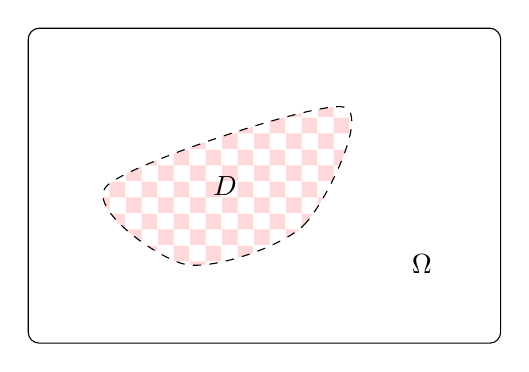
\begin{tikzpicture}
	\draw[rounded corners] (0,0) rectangle (6,4);
	\draw (5,1) node {$\Omega$};
	\draw[missing] plot[smooth cycle] coordinates {(2,1) (3.5,1.5) (4,3) (1,2)};
	\draw (2.5,2) node {$D$};
    \end{tikzpicture}
    \caption{Typische Inpainting-Situation}
    \label{fig:inpainting_setting}
\end{figure}

Beim Inpainten gehen wir von einem gegebenen Bild $u^0: \Omega \setminus D \to [0,1]$ und einem \emphdef{Inpainting-Bereich}
$D \subset \Omega$ aus (siehe Abbildung \ref{fig:inpainting_setting}). Ziel ist es nun eine Rekonstruktion $u: \Omega \to [0,1]$ zu finden, die optisch „möglichst gut zu $u^0$ passt“.

Wir werden „möglichst gut“ durch die Minimierung eines Funktionals $E: u \mapsto \R$,
\begin{math}
    E[u] = \Eimg[u] + \Edat[u]
\end{math}
beschreiben.
Hierbei sind die Funktionale $\Edat$, $\Eimg$ modelliert durch ein sogenanntes Datenmodell (engl. “data model”) und einem Bildmodell (engl. “image prior model”) ersetzen.
Der Bayes'sche Ansatz liefert für diesen Ansatz eine schmackhafte Motivation.


\section{Das Bayes'sche Prinzip}

% TODO: fix!!
% TODO: Energiebegriff erklären

Es seien hier $I_\Omega$, $I_{\Omega \setminus D}$ endlich.
Dies ist beispielsweise der Fall, wenn $\Omega \subset \Z^d$ beschränkt und $F$ endlich ist.
Auf praktisch alle digitalen Bilder triftt diese Annahme zu, da in der Regel diese auf einem endlichen Raster $(x_i, y_j)_{i=1,j=1}^{n,m}$ durch die Angabe von Farbwerten $(u_{i,j})_{i=1,j=1}^{n,m}$ gegeben sind und der zugehörige Farbraum aus endlich vielen verschiedenen Farbwerten besteht.

\begin{samepage}
Geht man davon aus, dass das ursprüngliche, vollständige Bild auch tatsächlich existiert, so lässt sich daraus die Entstehung der Beobachtung $u^0$ durch ein zweistufiges Zufallsexperiment modellieren.
\begin{enumerate}
    \item
	Zunächst tritt $u$ als Ereignis eines Zufallsexperiments auf, welches im (diskreten) Wahrscheinlichkeitsraum $(I_\Omega, 2^{I_\Omega}, P_{\mathrm{img}})$ modelliert wird. \nopagebreak
    \item
	Anschließend entsteht von $u$ auf $\Omega \setminus D$ eine Beobachtung $u^0$, welche ebenfalls als Zufallsexperiment modelliert wird,
	hier in $(I_{\Omega \setminus D}, 2^{I_{\Omega \setminus D}}, P_{\mathrm{dat},u})$.
\end{enumerate}
\end{samepage}
Wir betrachten dazu den diskreten Wahrscheinlichkeitsraum $\scr P := (I_\Omega \times I_{\Omega\setminus D}, 2^{I_\Omega \times I_{\Omega\setminus D}}, P)$ mit der sogenannten A-Posteriori-Wahrscheinlichkeitsverteilung
\begin{math}
    P(u, u^0) := P_{\mathrm{img}}(u) \cdot P_{\mathrm{dat},u^0}(u)
\end{math}
In diesem Raum besitzt $P_{\mathrm{dat},u^0}(u)$ die gewünschte Interpretation als bedingte Wahrscheinlichkeit $P(u^0|u)$:
\begin{math}
    P(u) &= P_{\mathrm{img}}(u), \\
    P(u^0|u) &= \frac{P(u, u^0)}{P(u)} = P_{\mathrm{dat},u^0}(u),
\end{math}
wobei wir $u$ und $u^0$ mit $\Set{u} \times I_{\Omega \setminus D}$, bzw. $I_\Omega \times \Set{u_0}$ identifizieren.
Dieser Raum erlaubt uns die Berechnung der bedingten Wahrscheinlichkeit
\begin{math}
    P(u|u^0) &= \frac{P(u, u^0)}{P(u^0)}
    = \frac{P(u^0|u) \cdot P(u)}{P(u^0)}.
\end{math}
Dieser einfache Zusammenhang zwischen den bedingten Wahrscheinlichkeiten ist auch als \emph{Satz von Bayes} bekannt.

Beim Inpainten ist $P(u^0)$ ist konstant und $P(u|u^0)$ die Wahrscheinlichkeit, dass $u$ die korrekte Rekonstruktion von $u^0$ ist, also maximieren wir
\begin{math}
    P(u|u^0) = \const \cdot P_{\mathrm{dat},u^0}(u) \cdot P_{\mathrm{img}}(u).
\end{math}
Wir können nun auf beiden Seiten $-\log(\argdot)$ anwenden und ein äquivalentes, aber durchaus handlicheres Problem in Energie-Form betrachten.

Für gegebenes $u^0$, $D$ minimieren wir also die Summe aus Datenterm und Bildterm (die additive Konstante ist für das Minimieren irrelevant)
\begin{math}
    E[u] = \Edat[u] + \Eimg[u].
\end{math}
Die Wahlen von $\Edat[u]$ und $\Eimg[u]$, welche den Wahrscheinlichkeitsverteilungen in unserem zweistufigen Zufallsmodell entsprechen, sind durch das Datenmodell, bzw. das Bildmodell festgelegt.


\section{Das Datenmodell}

Naheliegend ist der Gedanke, als Datenmodell lediglich $u|_{\Omega \setminus D} = u^0|_{\Omega \setminus D}$ zu fordern.
Damit würden feste Randbedingungen für das Minimieren auf $D$ vorgegeben werden.
In der Praxis sind Bilder jedoch meist mit Rauschen, Unschärfe oder anderen Artefakten versehen.
Dies kann z.B. durch technische Aufnahmebedingungen, natürlichen Zerfall oder durch digitale Kompressionsartefakte verursacht worden sein.
Das Datenmodell erlaubt es zu definieren, auf welche Weise $u|_{\Omega \setminus D}$ beim Inpainten an das vorliegende Bild $u^0$ angepasst werden soll und ermöglicht es solche Verunreinigungen auszugleichen.

Erwähnenswerterweise reduziert sich das Inpaintingproblem für $D = \emptyset$ auf das reine Ausgleichen dieser Verunreinigungen.
Somit kann z.B. das Entrauschen von Bildern (auch „Denoising“ genannt) als Spezialfall angesehen werden.

Für unser Datenmodell nutzen wir das bekannte Funktional aus \cite{rudin1992nonlinear}, welcher die quadrierte $L^2$-Norm verwendet:
\begin{math}
    \Edat[u] = \frac{\eta}{2} \int_{\Omega \setminus D} |u - u^0|^2,
\end{math}
wobei $\eta \in \R_{> 0}$ die spätere Gewichtung dieses Datenterms zum Bildterm kontrolliert.

Es ist bekannt \cite[§4.5]{chan2005image}, dass dieser Datenterm gut geeignet ist, wenn das Orginalbild mit Gauß'schem Rauschen versetzt ist, modelliert als $u^0 = u|_{\Omega \setminus D} + \epsilon$.
Für Schwarz/Weiß Rauschen (auch “salt-and-pepper noise” gennant) ist die Wahl einer $L^1$-Norm zu bevorzugen, wie in \cite{nikolova2004variational} gezeigt.

Denkbar wären auch Datenmodelle wie $u^0 = K[u|_{\Omega\setminus D}] + \epsilon$ für einen Glättungsoperator $K$.
Solche Modelle würden es erlauben, Unschärfe zu reduzieren, siehe z.B. \cite{rudin1994total}.


\section{Das Bildmodell}

Da der Datenterm sich auf $\Omega \setminus D$ beschränkt hat, trägt das Bildmodell die Hauptrolle bei der eigentlichen Bildrekonstruktion innerhalb von $D$.
Man beachte, dass das Bildmodell unabhängig von $D$ ist (man erinnere sich an das Bayes-Prinzip) und auch für den Fall $D = \emptyset$ (z.B. Denoising) die Rekonstruktion des ursprünglichen Bildes verbessern kann.
In der Literatur zum Denoising wird $\Eimg[u]$ manchmal auch als „regularization term” bezeichnet.

\begin{figure}[ht]
    \begin{subfigure}[b]{0.33\textwidth}
	\centering
        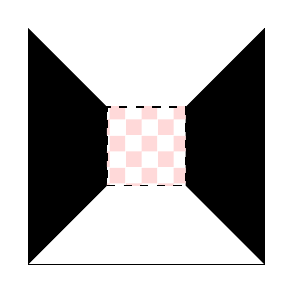
\begin{tikzpicture}
	    \draw[clip] (0,0) rectangle (3,3);
	    \fill[bg] (0,0) rectangle (3,3);
	    \fill[fg] (0,0) -- (1,1) -- (1,2) -- (0,3) -- cycle;
	    \fill[fg] (3,0) -- (3,3) -- (2,2) -- (2,1) -- cycle;
	    \draw[missing] (1,1) -- (2,1) -- (2,2) -- (1,2) -- cycle;
        \end{tikzpicture}
    \end{subfigure}%
    \begin{subfigure}[b]{0.33\textwidth}
	\centering
        
\begin{tikzpicture}
	    \draw[clip] (0,0) rectangle (3,3);
	    \fill[fg] (0,0) rectangle (3,3);
	    \fill[bg] (0,0) -- (3,0) -- (2,1) -- (1,1) -- cycle;
	    \fill[bg] (0,3) -- (1,2) -- (2,2) -- (3,3) -- cycle;
        \end{tikzpicture}
    \end{subfigure}%
    \begin{subfigure}[b]{0.33\textwidth}
	\centering
        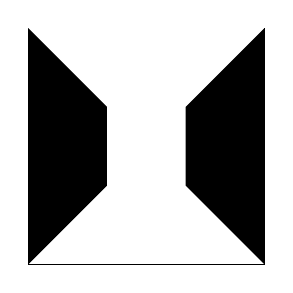
\begin{tikzpicture}
	    \draw[clip] (0,0) rectangle (3,3);
	    \fill[bg] (0,0) rectangle (3,3);
	    \fill[fg] (0,0) -- (1,1) -- (1,2) -- (0,3) -- cycle;
	    \fill[fg] (3,0) -- (3,3) -- (2,2) -- (2,1) -- cycle;
        \end{tikzpicture}
    \end{subfigure}
    \caption{Bewertungsschwierigkeiten: welches der beiden vollständigen Bildern ist wahrscheinlicher?}
    \label{fig:inpainting_non_unique}
\end{figure}

Zunächst macht man sich schnell anhand von einfachen Beispielen klar, dass die Wahl eines guten Bildmodells keineswegs einfach oder eindeutig ist, da die Bildbewertung oft von der menschlichen Interpretation abhängt.
Welche der beiden vollständigen Bilder aus Abbildung \ref{fig:inpainting_non_unique} ein Betrachter eher für richtig hält, hängt davon ab, ob er Hell oder Dunkel für vordergründiger hält.

\begin{figure}[ht]
    \begin{subfigure}[b]{0.33\textwidth}
	\centering
        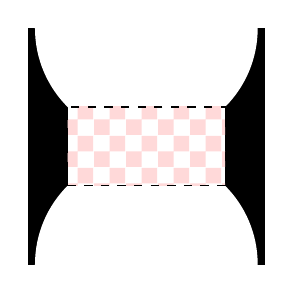
\begin{tikzpicture}
	    \draw[clip] (0,0) rectangle (3,3);
	    \fill[fg] (0,0) rectangle (3,3);
	    \fill[bg] (1.5,3) circle[radius=1.41421];
	    \fill[bg] (1.5,0) circle[radius=1.41421];
	    \fill[bg] (0.5,1) -- (2.5,1) -- (2.5,2) -- (0.5,2) -- cycle;
	    \draw[missing] (0.5,1) -- (2.5,1) -- (2.5,2) -- (0.5,2) -- cycle;
        \end{tikzpicture}
    \end{subfigure}%
    \begin{subfigure}[b]{0.33\textwidth}
	\centering
        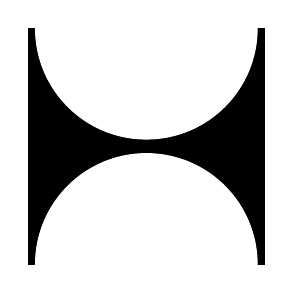
\begin{tikzpicture}
	    \draw[clip] (0,0) rectangle (3,3);
	    \fill[fg] (0,0) rectangle (3,3);
	    \fill[bg] (1.5,3) circle[radius=1.41421];
	    \fill[bg] (1.5,0) circle[radius=1.41421];
        \end{tikzpicture}
    \end{subfigure}%
    \begin{subfigure}[b]{0.33\textwidth}
	\centering
        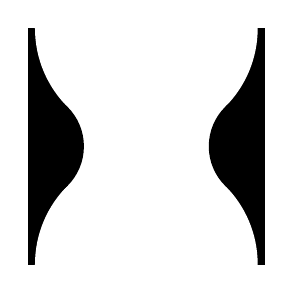
\begin{tikzpicture}
	    \draw[clip] (0,0) rectangle (3,3);
	    \fill[fg] (0,0) rectangle (3,3);
	    \fill[bg] (1.5,3) circle[radius=1.41421];
	    \fill[bg] (1.5,0) circle[radius=1.41421];
	    \fill[bg] (0.5,1) -- (2.5,1) -- (2.5,2) -- (0.5,2) -- cycle;
	    \fill[fg] (0,1.5) circle[radius=0.70710];
	    \fill[fg] (3,1.5) circle[radius=0.70710];
        \end{tikzpicture}
    \end{subfigure}
    \caption{Lösungen eines Inpaintingproblems (links) mit langen (mitte) und kurzen (rechts) Niveaulinien}
    \label{fig:inpainting_prefer_short}
\end{figure}

%\begin{figure}[ht]
%    \begin{subfigure}[b]{0.33\textwidth}
%	\centering
%        \begin{tikzpicture}
%	    \draw[clip] (0,0) rectangle (3,3);
%	    \fill[fg] (0,0) rectangle (3,3);
%	    \fill[bg] (1.5,3) circle[radius=1.11803];
%	    \fill[bg] (1.5,0) circle[radius=1.11803];
%	    \fill[bg] (1,1) -- (2,1) -- (2,2) -- (1,2) -- cycle;
%	    \draw[missing] (1,1) -- (2,1) -- (2,2) -- (1,2) -- cycle;
%        \end{tikzpicture}
%    \end{subfigure}%
%    \begin{subfigure}[b]{0.33\textwidth}
%	\centering
%        \begin{tikzpicture}
%	    \draw[clip] (0,0) rectangle (3,3);
%	    \fill[fg] (0,0) rectangle (3,3);
%	    \fill[bg] (1.5,3) circle[radius=1.11803];
%	    \fill[bg] (1.5,0) circle[radius=1.11803];
%        \end{tikzpicture}
%    \end{subfigure}%
%    \begin{subfigure}[b]{0.33\textwidth}
%	\centering
%        \begin{tikzpicture}
%	    \draw[clip] (0,0) rectangle (3,3);
%	    \fill[fg] (0,0) rectangle (3,3);
%	    \fill[bg] (1.5,3) circle[radius=1.11803];
%	    \fill[bg] (1.5,0) circle[radius=1.11803];
%	    \fill[bg] (1,1) -- (2,1) -- (2,2) -- (1,2) -- cycle;
%	    \fill[fg] (0.75,1.5) circle[radius=0.55902];
%	    \fill[fg] (2.25,1.5) circle[radius=0.55902];
%        \end{tikzpicture}
%    \end{subfigure}
%    \caption{Krümmungsarme Niveaulinien (mitte) werden bevorzugt}
%    \label{fig:inpainting_prefer_non_curved}
%\end{figure}

\begin{figure}[ht]
    \begin{subfigure}[b]{0.33\textwidth}
	\centering
        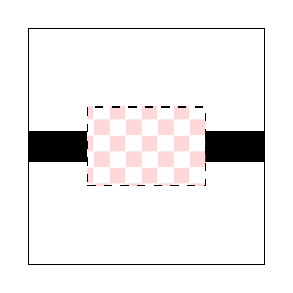
\begin{tikzpicture}
	    \draw[clip] (0,0) rectangle (3,3);
	    \fill[fg] (0,1.3) rectangle (3,1.7);
	    \fill[bg] (0.75,1) -- (2.25,1) -- (2.25,2) -- (0.75,2) -- cycle;
	    \draw[missing] (0.75,1) -- (2.25,1) -- (2.25,2) -- (0.75,2) -- cycle;
        \end{tikzpicture}
    \end{subfigure}%
    \begin{subfigure}[b]{0.33\textwidth}
	\centering
        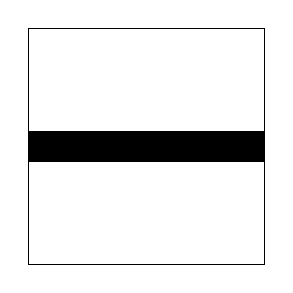
\begin{tikzpicture}
	    \draw[clip] (0,0) rectangle (3,3);
	    \fill[fg] (0,1.3) rectangle (3,1.7);
        \end{tikzpicture}
    \end{subfigure}%
    \begin{subfigure}[b]{0.33\textwidth}
	\centering
        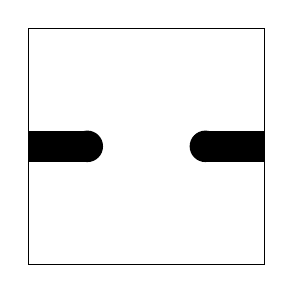
\begin{tikzpicture}
	    \draw[clip] (0,0) rectangle (3,3);
	    \fill[fg] (0,1.3) rectangle (3,1.7);
	    \fill[bg] (0.75,1) -- (2.25,1) -- (2.25,2) -- (0.75,2) -- cycle;
	    \fill[fg] (0.75,1.5) circle[radius=0.2];
	    \fill[fg] (2.25,1.5) circle[radius=0.2];
        \end{tikzpicture}
    \end{subfigure}
    \caption{Lösungen eines Inpaintingproblems (links) mit Nivaulinien ohne Krümmung (mitte) und Niveaulinien höherer Krümmung (rechts)}
    \label{fig:inpainting_prefer_non_curved}
\end{figure}

Wir betrachten nun zweidimensionale Bilder $d = 2$.
Ohne entsprechende Studien durchgeführt zu haben, kann man anhand von Abbildungen \ref{fig:inpainting_prefer_short} und \ref{fig:inpainting_prefer_non_curved} erahnen, dass Bilder, bei denen die Kanten (oder Niveaulinien) des Bildes möglichst kurz und gering gekrümmt sind, ästhetisch angenehmer\footnote{Der Autor bevorzugt in Abbildung \ref{fig:inpainting_prefer_short} das rechte Bild und in Abbildung \ref{fig:inpainting_prefer_non_curved} das mittlere Bild}.

Die Niveaulinien stellen auf diese Weise eine brauchbare Bewertungsgrundlage eines Bildes dar.
Legt man nun eine geeignete Bewertung für die Niveaulinien eines Bildes (im Sinne eines Energiefunktionals) fest, so liefert die Summation über alle Höhenlinien eine Bewertung des Gesamtbildes.
Die sogenannte \emphdef{Levelset-Methode} in Kapitel \ref{chap:image_model} erlaubt die Umsetzung dieser Idee.

Das Bildmodell in dieser Arbeit nutzt die Levelset-Methode und wählt für jede Niveaulinie $\gamma:[0,1] \to \Omega$ die \emphdef{Elastica Energie}
\begin{math}
    \int_{\gamma} \alpha + \beta \kappa^2 \di[s]
\end{math}
als Kurvenintegral über $\gamma$ mit festen Parametern $\alpha, \beta \in \R_{\ge 0}$, wobei $\kappa: [0,1] \to \R$ die parametrisierte Krümmung von $\gamma$ darstellt.

Eine Kurve, die diese Energie (unter geeigneten Randbedingungen) minimiert, wird \emphdef{Elastica} genannt.
In der Physik hat sie die Interpretation der Biegeenergie eines elastischen Stabes.
Umfangreiche Herleitungen finden sich in \cite{love1920treatise} und \cite{antman2005problems}, während obige Form der Elastica Energie aus \cite{birkhoff1965nonlinear} stammt.

Die Levelset-Methode liefert uns schließlich für unser Bildmodell (näheres in Kapitel \ref{chap:image_model})
\begin{math}
    \Eimg[u] = \int_{\Omega} \Big(\alpha + \beta (\nabla \cdot \frac{\nabla u}{\nabla u})^2\Big)|\nabla u| \di[x],
\end{math}
wobei der Term $\nabla \cdot \frac{\nabla u}{|\nabla u|}$ die Krümmung der Niveaulinie im entsprechenden Punkt darstellt.
Mit Blick auf \ref{fig:inpainting_texture} sei bemerkt, dass dieses geometrische Inpaintingmodell nicht darauf ausgelegt ist, wiederkehrende Strukturen zu reproduzieren, die deutlich kleiner als der Inpaintingbereich $D$ sind.
Die Minimierung einer Energie basierend auf Niveaulinien und der Levelset-Methode ist in diesem Fall nicht zielführend, da sie eine zu lokale Methode darstellt.
Um solche Strukturen oder Texturen zu rekonstruieren, müssen größere Teile des Bildes in Betracht gezogen werden.
Hierfür gibt es das sogenannte “texture based inpainting” mit zahlreichen stochastischen Methoden (siehe z.B. \cite{criminisi2004region}).

\begin{figure}[ht]
    \begin{subfigure}[b]{0.33\textwidth}
	\centering
        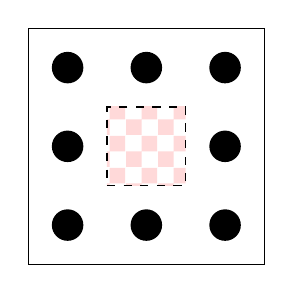
\begin{tikzpicture}
	    \draw[clip] (0,0) rectangle (3,3);
	    \foreach \x in {0.5, 1.5, 2.5}
		\foreach \y in {0.5, 1.5, 2.5}
		    \fill (\x,\y) circle[radius=0.2];
	    \fill[bg] (1,1) -- (2,1) -- (2,2) -- (1,2) -- cycle;
	    \draw[missing] (1,1) -- (2,1) -- (2,2) -- (1,2) -- cycle;
        \end{tikzpicture}
    \end{subfigure}%
    \begin{subfigure}[b]{0.33\textwidth}
	\centering
        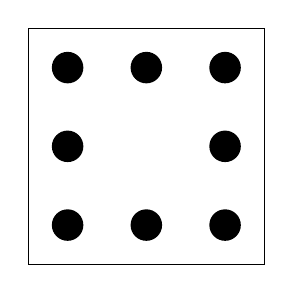
\begin{tikzpicture}
	    \draw[clip] (0,0) rectangle (3,3);
	    \foreach \x in {0.5, 1.5, 2.5}
		\foreach \y in {0.5, 1.5, 2.5}
		    \fill (\x,\y) circle[radius=0.2];
	    \fill[bg] (1,1) -- (2,1) -- (2,2) -- (1,2) -- cycle;
        \end{tikzpicture}
    \end{subfigure}%
    \begin{subfigure}[b]{0.33\textwidth}
	\centering
        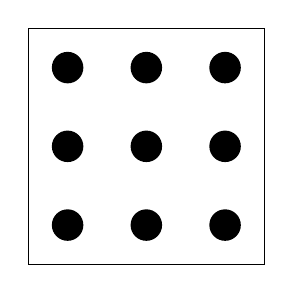
\begin{tikzpicture}
	    \draw[clip] (0,0) rectangle (3,3);
	    \foreach \x in {0.5, 1.5, 2.5}
		\foreach \y in {0.5, 1.5, 2.5}
		    \fill (\x,\y) circle[radius=0.2];
        \end{tikzpicture}
    \end{subfigure}
    \caption{Unser Bildmodell würde das mittlere Bild dem rechten vorziehen}
    \label{fig:inpainting_texture}
\end{figure}


\chapter{Technische Hilfsmittel und Konventionen}


\section*{Konventionen}

Um die Notation zu erleichtern, werden wir eine Reihe von Konventionen befolgen, die Folgenden festgehalten werden sollen.

\begin{itemize}
    \item
	Jedes Auftreten von „$\const$“ bezeichnet eine neue, nicht näher definierte Konstante im entsprechenden Raum.
	In der Regel ist $\const \in \R_{>0}$.
    \item
	Bei Integralen einer Funktion $f: X \to Y$ über Teilmengen des Definitionsbereiches von $f$ wird das Funktionsargument ausgespart, z.B. $\int_X f \dx$.
    \item
	Bei Integralen über Teilmengen des $\R^d$ wird das Integrationsmaß ausgespart, falls es sich um das übliche Lebesgue-Maß handelt.
    \item
	Für Vektoren $v, w \in \R^d$ bezeichnen wir mit $v \cdot w$ das euklidische Skalarprodukt von $v$ und $w$ und mit $|v|$ die euklidische Norm von $v$.
    \item
	Für Funktionen $f, g \in H$ eines Hilbertraums $H$ bezeichen wir mit $\<f, g\>$ das zugehörige Skalarprodukt von $f$ und $g$ und mit $\|f\|$ die entsprechende Norm von $f$.
    \item
	Für Funktionen $f, g: X \to \R^d$ bezeichnen wir mit $f \cdot g$ das punktweise Skalarprodukt $f \cdot g: x \mapsto f(x)\cdot g(x)$ und mit $|f|$ die punktweise euklidische Norm $|f|: x \mapsto |f(x)|$.
    \item
	Für einen Hilbertraum $H$ bezeichnen wir Funktionen $I: H \to \R$ als \emphdef{Funktionale} und schreiben ihr Argument stets in eckigen Klammern: $I[f] \in \R$ für $f \in H$.
\end{itemize}


\section*{Differentialgeometrie}


\section*{Optimierung}

Wir nutzen in Kapitel \ref{chap:ee} und \ref{chap:ad} Variationsrechnung im Zusammenhang mit Optimierung und führen dazu kurz die nötigen Werkzeuge ein.
Im Folgenden sei $H$ stets ein Hilbertraum.

\begin{definition} \label{definition:min_stuff}
    Wir nennen $I: H \to \R$
    \begin{itemize}
	\item
	    \emphdef{Gateaux-differenzierbar},
            falls für alle $u, \phi \in H$ das \emphdef{Gateaux-Differential $I': H \times H \to \R$ von $I$ an der Stelle $u$ in Richtung $\phi$}
	    \begin{math}
		I'[u, \phi]
		:= \ddx[\epsilon]|_{\epsilon = 0} I[u + \epsilon \phi]
		= \lim_{\delta \to 0} \dfrac{I[u + \delta \phi] - I[u]}{\delta}
	    \end{math}
	    existiert und $I'[u, \argdot]: H \to \R$ ein linearer und beschränkter Operator ist,
        \item
	    \emphdef{konvex},
	    falls für alle $u_1, u_2 \in H$, $t \in [0,1]$ gilt
	    \begin{math}
		I[t u_1 + (1-t) u_2]
		\le tI[u_1] + (1-t)I[u_2],
	    \end{math}
	\item
	    \emphdef{koerziv},
	    falls für jede Folge $(u_k)_{k\in\N}$ gilt
	    \begin{math}
		\|u_k\| \to \infty \implies I(u_k) \to \infty.
	    \end{math}
    \end{itemize}
\end{definition}

Folgender einfache Satz rechtfertigt das Ermitteln von kritischen Punkten eines Funktionals um sein Minimum zu bestimmen.

\begin{proposition} \label{proposition:min_zero}
    Sei $\hat u \in H$ und $I: H \to \R$ Gâteaux-differenzierbar und konvex.
    Dann gilt
    \begin{math}
        I[\hat u] = \inf_{u \in H} I[u]
	\iff
	\forall \phi \in H : I'[\hat u, \phi] = 0.
    \end{math}
    \begin{note}
	Über die Lösbarkeit von $I'[u, \phi] = 0$ für alle $\phi$, bzw. die Existenz des Minimums $\hat u$ wird hier keine Aussage getroffen, siehe dazu Theorem \ref{theorem:min_existence}.
    \end{note}
    \begin{proof}
	„$\implies$”: Sei $I[\hat u] \le I[u]$ für alle $u \in H$.
	Dann gilt für alle $\phi \in H$
	\begin{math}
	    I'[\hat u, \phi] = \lim_{\epsilon \to 0} \frac{I[\hat u + \epsilon \phi] - I[\hat u]}{\epsilon}
	    \ge 0,
	\end{math}
	also auch $-I'[\hat u, \phi] = I'[\hat u, -\phi] \ge 0$ und somit $I'[\hat u, \phi] = 0$.

	„$\impliedby$”: Sei $I'[\hat u, \phi] = 0$ für alle $\phi \in H$.
	Wegen Konvexität haben wir
	\begin{math}
	    0 = I'[\hat u, u - \hat u]
	    &= \lim_{\epsilon \to 0} \frac{1}{\epsilon} \big( I[\epsilon u + (1-\epsilon) \hat u] - I[\hat u] \big) \\
	    &\le \lim_{\epsilon \to 0} \frac{1}{\epsilon} \big( \epsilon I[u] + (1- \epsilon) I[\hat u] - I[\hat u] \big) \\
	    &= I[u] - I[\hat u],
	\end{math}
	also $I[\hat u] \le I[u]$ für alle $u \in H$.
    \end{proof}
\end{proposition}

\begin{theorem} \label{theorem:min_existence}
    Sei $H$ ein Hilbertraum, $I: H \to \R$ Gateaux-differenzierbar, konvex und koerziv.
    Dann existiert ein Minimum $\hat u \in H$, d.h.
    \begin{math}
        I[\hat u] = \inf_{u \in H} I[u].
    \end{math}
    \begin{proof}
        Ein Beweis für eine etwas allgemeinere Version findet sich in \cite[Theorem 7.3.8]{kurdila2006convex}.
    \end{proof}
\end{theorem}

Die obigen beiden Aussagen sind für die Minimierung von konvexen Funktionalen von wesentlicher Bedeutung.
Zur Untersuchung der nötigen Voraussetzungen für spätere Zwecke folgen zwei einfache, konkretere Lemmata.

\begin{proposition} \label{proposition:convexity}
    Für Funktionale $I: H \to \R$ gelten folgende Aussagen über ihre Konvexität.
    \begin{enumerate}[i)]
	\item
	    Konstante Funktionale sind konvex.
	\item
	    Lineare Funktionale sind konvex.
        \item
	    Die (punktweise) Summe zweier konvexer Funktionale ist konvex.
	\item
	    Seien $\Omega \subset \R^d$ und $H := L^2(\Omega)^d$.
	    Seien $A: H \to H$ ein linearer Operator, $v \in H$ und $w \in L^1(\Omega)$ sodass $w|Au + v|^2 \in L^1(\Omega)$.
	    Dann ist das Funktional
	    \begin{math} %FIXME: w is bad, make it more general?
	        I: u \mapsto \int_\Omega w|Au + v|^2
	    \end{math}
	    konvex.
    \end{enumerate}
    \begin{proof}
	Die Aussagen i), ii) und iii) sind mit Blick auf Definition \ref{definition:min_stuff} sofort ersichtlich, wir zeigen nur iv).

	Sei $I: u \mapsto \int_\Omega w|Au + v|^2$ für einen linearen Operator $A$.
	Wegen
	\begin{math}
	    |Au - v|^2
	    = |Au|^2 - 2Au \cdot v + |v|^2
	\end{math}
	genügt es mit Blick auf i), ii) und iii) den Fall $v = 0$ zu betrachten.
	Es folgt mit $t^2 = t - t(1-t)$ punktweise
	\begin{math}
	    |A(tu_1 + (1-t)u_2)|^2
	    &= t^2 |Au_1|^2 - 2 t(1-t) Au_1\cdot Au_2 + (1-t^2)|Au_2|^2 \\
	    &= t|Au_1|^2 - t(1-t)\underbrace{\big(|Au_1|^2 - 2Au_1 \cdot Au_2 + |Au_2|^2\big)}_{=|A(u_1 - u_2)|^2 \ge 0} + (1-t)|Au_2|^2 \\
	    &\le t|Au_1|^2 + (1-t)|Au_2|^2,
	\end{math}
	also wegen Distributivität der Multiplikation und Linearität des Integrals auch $I[tu_1 + (1-t)u_2] \le tI[u_1] + (1-t)I[u_2]$.
    \end{proof}
\end{proposition}

\begin{proposition} \label{proposition:coercivity}
    Für Funktionale $I: H \to \R$ gelten folgende Aussagen über ihre Koerzivität:
    \begin{enumerate}[i)]
        \item
	   Die (punktweise) Summe zweier koerziver Funktionale ist koerziv.
       \item
	   Sei $I: H \to \R$ koerziv und $J: H \to \R$ nach unten beschränkt.
	   Dann ist $I + J$ koerziv.
       \item
	   Seien $\Omega \subset \R^d$, $H := L^2(\Omega)^d$, $v, w \in H$.
	   Dann ist das Funktional
	   \begin{math}
	       I: u \mapsto \int_\Omega |u - v|^2 + \int_\Omega u \cdot w
	   \end{math}
	   koerziv.
    \end{enumerate}
    \begin{proof}
	Die Aussagen i) und ii) sind mit Blick auf Definition \ref{definition:min_stuff} leicht ersichtlich und wir zeigen nur iii).
	Durch quadratische Ergänzung und mit Hilfe von ii) genügt es den Fall $w = 0$ zu betrachten.
	Hierfür ist
	\begin{math}
	    I[u] = \int_\Omega |u - v|^2 = \|u - v\|^2 \ge (\|u\| - \|v\|)^2,
	\end{math}
	also für eine Folge $\|u_k\| \to \infty$ auch $I[u_k] \to \infty$.
    \end{proof}
\end{proposition}







\chapter{Das Euler Elastica Bildmodell} \label{chap:image_model}


Wir bereits in der Einführung angesprochen, wollen wir in diesem Kapitel die Elastica Kurve als Kurvenmodell für die Niveaulinien eines Bildes ansetzen, um daraus anschließend ein Bildmodell zu gewinnen.
Obwohl das hieraus gewonnene Bildmodell später auch für $d > 2$ interpretiert werden kann (siehe \ref{thm:eemodel}), werden wir uns für die Herleitung auf die Dimension $d = 2$ festlegen.

\section{Die Euler Elastica}

In der Physik bezeichnet man einen festen Gegenstand in der Regel als elastisch, wenn er sich unter äußerer Krafteinwirkung deformiert und nach dem Entfernen dieser Kraft wieder in seine Ausgangsform zurückkehrt.
Die Frage, wie genau sich ein elastischer Gegenstand unter äußerer Krafteinwirkung verformt, ist im Allgemeinen stark materialabhängig und schwierig zu beantworten.

Die Wissenschaft hat mit der Zeit eine Reihe von Modellen entwickelt, um das Verhalten elastischer Gegenstände zu beschreiben.
Man erinnere sich beispielsweise an das Hookesche Gesetz aus der Schulphysik, welches zwischen Elongation eines Objektes (z.B. eine Spannfeder) in eine Richtung und der darauf einwirkenden Kraft einen linearen Zusammenhang herstellt.
Dieses Modell war jedoch eindimensional und reichte auch nicht aus, um größere Verformungen zu beschreiben, die sich nicht dem linearen Gesetz unterwerfen.

Euler hat schließlich (nach Vorarbeit von Bernoulli und anderen, siehe \cite{levien2008elastica}) 1744 in seinem Buch über variationelle Methoden \cite{euler1774methodus} ein Modell für planare elastische Stäbe fester Länge präsentiert.
Eine Elastica war demnach (in aktueller Notation) eine zweifach stetig differenzierbare, reguläre Kurve $\gamma: [0,L] \to \R^2$ fester Länge $L > 0$, festen Endpunkten $\gamma(0), \gamma(L)$ und festen Tangentenrichtungen $\dot \gamma(0), \dot \gamma(L)$, welche die totale quadrierte Krümmung
\begin{math}
    \int_\gamma \kappa^2 \di[s]
\end{math}
minimiert.
In seinem Werk löst Euler dieses Variationsproblem indem er alle zugehörigen kritischen Punkte (Kurven) klassifiziert und weist darauf hin, dass das Modell bekannte Eigenschaften elastischer Stäbe reproduziert.

Neben ihrer geschmeidigen Form erbt die Elastica durch diese Formulierung auch viele schöne geometrische Eigenschaften der Krümmung, wie z.B. Invarianz unter euklidischen Transformationen.
In neuerer Zeit wurde die Elastica deshalb in der Numerik z.B. als Vorbild für Spline-Interpolationen oder – wie in dieser Arbeit – als Kurvenmodell für Levelsetmethoden in Betracht gezogen.
Man möchte sich dabei meist von der unhandlichen Randbedingung der festen Länge befreien und wählt folgende Definition.

\begin{definition}[Euler Elastica] \label{definition:elastica}
    Seien $\alpha, \beta \in \R_{\ge 0}$.
    Eine Kurve $\gamma \in C^2([0,1], \R^2)$ mit festen Endpunkten $\gamma(0) = p_0$, $\gamma(1) = p_1$ und Tangentenrichtungen $\dot\gamma(0) = t_0$, $\dot\gamma(1) = t_1$ heißt \emphdef{Elastica}, falls sie unter eben solchen zulässigen Kurven ein kritischer Punkt des Energiefunktionals
    \begin{math}
	\int_\gamma \alpha + \beta \kappa^2 \di[s]
    \end{math}
    ist.
    Diese Energie nennen wir auch \emphdef{Elastica Energie der Kurve $\gamma$}.
    \begin{note}
	Das Verhältnis $\frac{\beta}{\alpha}$ bestimmt die Art der Kurve: für kleines $\frac{\beta}{\alpha}$ werden kürzere Verbindungsstrecken bevorzugt, während größeres $\frac{\beta}{\alpha}$ scharfe Kurven vermeidet und ein glatteres Gesamtbild erzeugt.
	In Kapitel \ref{chap:numerics} wird diese Eigenschaft am zugehörigen Inpaintingresultat sichtbar.
    \end{note}
\end{definition}

Eine interessante Charakterisierung der Elastica liefert der folgende Satz.

\begin{proposition} \label{proposition:elastica_el}
    Eine Kurve $\gamma \in C^4([0,1], \R^2)$ mit Randbedingungen wie in Definition \ref{definition:elastica} ist eine Elastica genau dann, wenn die zugehörige Euler-Lagrange-Gleichung für die Krümmung
    \begin{math}
	\beta\big(2\ddot\kappa + \kappa^3\big) = \alpha\kappa
    \end{math}
    erfüllt ist.
    \begin{proof}
	Sei $\gamma:[0,L] \to \R^2$ in Bogenlänge parametrisiert und ebenso ihre Tangente $e_1$, Normale $e_2$ und Krümmung $\kappa$.
        Die Kurvenenergie sei gegeben durch $I[\gamma] := \int_\gamma \alpha + \beta \kappa^2 \di[s]$.
	Wir bedienen uns der Variationsrechnung und lösen
	\begin{math}
	    \ddx[\epsilon]|_{\epsilon=0} I[\gamma + \epsilon \phi e_2] = 0,
	\end{math}
	wobei $\phi \in C^2([0,L], \R^2)$ eine Variation in Normalenrichtung $e_2$ darstellt.
	Sei $\gamma_\epsilon = \gamma + \epsilon \phi e_2$.
	Die Krümmung $\kappa_\epsilon$ von $\gamma_\epsilon$ lässt sich parametrisierungsunabhängig durch $\kappa_\epsilon = \frac{\det(\dot\gamma_\epsilon, \ddot\gamma_\epsilon)}{|\dot\gamma_\epsilon|^3}$ darstellen.
	Wir berechnen nun
	\begin{math}
	    \dot \gamma_\epsilon &= e_1 + \epsilon \dot \phi e_2 - \epsilon \phi \kappa e_1 \\
	    &= (1-\epsilon \phi \kappa)e_1 + \epsilon \dot \phi e_2, \\
	    \ddot \gamma_\epsilon &= (-\epsilon \dot \phi \kappa - \epsilon \phi \dot \kappa) e_1 + (1-\epsilon \phi \kappa) \kappa e_2 + \epsilon \ddot \phi e_2 - \epsilon \dot \phi \kappa e_1 \\
	    &= (-2\epsilon \dot\phi \kappa - \epsilon \phi \dot \kappa) e_1 + (\epsilon \ddot \phi - \epsilon \phi \kappa^2 + \kappa) e_2, \\
	    \det(\dot\gamma_\epsilon, \ddot \gamma_\epsilon)
	    &=(1-\epsilon\phi\kappa)(\epsilon\ddot\phi - \epsilon\phi\kappa^2 + \kappa) + \epsilon \dot\phi(2 \epsilon \dot\phi \kappa - \epsilon\phi\dot\kappa),
	\end{math}
	und somit
	\begin{math}
	    \ddx[\epsilon]|_{\epsilon=0} |\dot\gamma_\epsilon|
	    &= \frac{1}{|\dot\gamma_0|} (\dot\gamma_0 \cdot \ddx[\epsilon] \dot\gamma_\epsilon) \\
	    &= e_1 \cdot (-\phi \kappa e_1 + \dot \phi e_2) \\
	    &= - \phi \kappa, \\
	    \ddx[\epsilon]|_{\epsilon=0} \det(\dot\gamma_\epsilon, \ddot\gamma_\epsilon)
	    &= -\phi \kappa^2 + (\ddot \phi - \phi\kappa^2) + \dot\phi \cdot 0 + 0 \cdot (2\dot\phi\kappa - \phi \dot\kappa) \\
	    &= \ddot\phi - 2\phi\kappa^2.
	\end{math}
	Zusammen ergibt sich
	\begin{math}
	    0 &= \ddx[\epsilon]|_{\epsilon = 0} I[\gamma_\epsilon] \\
	    &= \ddx[\epsilon]|_{\epsilon=0} \int_0^L (\alpha + \beta \kappa_\epsilon^2)|\dot\gamma_\epsilon|  \\
	    &= \int_0^L \alpha \ddx[\epsilon]|_{\epsilon = 0}|\dot\gamma_\epsilon| + \beta \ddx[\epsilon]|_{\epsilon = 0} \dfrac{\det(\dot\gamma_\epsilon, \ddot\gamma_\epsilon)^2}{|\dot\gamma_\epsilon|^5}  \\
	    &= \int_0^L -\alpha \kappa \phi + \beta \Big(2\kappa \ddx[\epsilon]|_{\epsilon=0} \det(\dot\gamma_\epsilon, \ddot\gamma_\epsilon) + 5\kappa^3 \phi \Big) \\
	    &= \int_0^L 2\beta\kappa \ddot\phi + \beta \kappa^3 \phi - \alpha\kappa\phi.
	\end{math}
	Zweimalige partielle Integration unter Beachtung der Randbedingungen $\phi(0), \phi(1), \dot\phi(0), \dot\phi(L) = 0$ liefert
	\begin{math}
	    0 &= \int_0^L \Big(2\ddot\kappa + \beta \kappa^3 - \alpha\kappa \Big) \phi
	\end{math}
	und mit dem Hauptsatz der Variationsrechnung also
	\begin{math}
	    \beta(2\ddot\kappa + \kappa^3) - \alpha \kappa = 0.
	\end{math}
    \end{proof}
\end{proposition}

%TODO: kinetische Betrachtung


\section{Die Levelset-Methode}

Die Idee der Levelset-Methode in der Numerik ist es, Berechnungen auf Kurven (oder Flächen) mit Hilfe einer sogenannten Levelset-Funktion in kartesischen Koordinaten durchführen zu können, ohne jeweils eine konkrete Parametrisierung der Kurven zu benötigen.
Die Levelset-Funktion enthält dabei die zu betrachtenden Kurven als Niveaulinien.

\begin{definition}
    Sei $\Omega \subset \R^2$ offen, $\gamma \in C^1([0,1], \Omega)$ eine reguläre Kurve und $\lambda \in \R$.
    Eine stetig differenzierbare Abbildung $u: \Omega \to \R^2$ heißt \emphdef{$\lambda$-Levelset-Funktion} für $\gamma$, falls für alle $t \in [0,1]$ gilt
    \begin{enumerate}[i)]
        \item
	    $(u \circ \gamma)(t) = \lambda$ und
	\item
	    $\det(\dot \gamma(t), \nabla u(\gamma(t))) > 0$.
    \end{enumerate}
    Wir nennen $\gamma$ auch \emphdef{$\lambda$-Levelset-Kurve} zu $u$.
    \begin{note}
        Die zweite Bedingung $\det(\dot \gamma, \nabla u) > 0$ sichert uns eine einheitliche Orienterung der Kurve.
    \end{note}
\end{definition}

Viele von $\gamma$ abhängige Größen können nun auch durch $u$ dargestellt werden, wie z.B. die Einheitsnormale $e_2$ von $\gamma$ an einem Punkt $x = \gamma(t)$.
Einmaliges Ableiten von $(u \circ \gamma)(t) = \lambda$ nach $t$ liefert nämlich
\begin{math}
    0 = \nabla u(\gamma(t)) \cdot \dot \gamma(t).
\end{math}
Falls $\nabla u(x) \neq 0$, so muss also $\frac{\nabla u(x)}{|\nabla u(x)|} = e_2(t)$, wobei das Vorzeichen durch $\det(\dot\gamma, \nabla u) > 0$ sichergestellt ist.
Dies motiviert folgende Definition.

\begin{definition}
    Für eine Abbildung $u \in C^1(\Omega, [0,1])$ mit $\nabla u(x) \neq 0$ für alle $x \in \Omega$ sei
    \begin{math}
        n: \Omega &\to \R^2 \\
	x &\mapsto \frac{\nabla u(x)}{|\nabla u(x)|}
    \end{math}
    das \emphdef{Normalenfeld} von $u$.
\end{definition}

Die Elastica Energie $\int_\gamma \alpha + \beta \kappa^2 \di[s]$ im Hinterkopf, wollen wir nun die Krümmung $\kappa$ der Niveaulinie eines Bildes durch $u$ darstellen.

\begin{lemma}
    Sei $\Omega \subset \R^2$, $\gamma \in C^2([0,1], \Omega)$ regulär und $u \in C^2(\Omega, [0,1])$ eine zugehörige Levelset-Funktion mit Normalenfeld $n: \Omega \to \R^2$ und $\nabla u \neq 0$ auf $\Omega$.
    Dann gilt für alle $t \in [0,1]$, $x := \gamma(t)$
    \begin{math}
	\kappa(t) = - \nabla \cdot n(x) = - \nabla \cdot \frac{\nabla u(x)}{|\nabla u(x)|}.
    \end{math}
    \begin{note}
	Allgemeiner beschreibt $-\nabla \cdot n$ in der Differentialgeometrie die mittlere Krümmung einer Fläche mit Normale $n$, siehe \cite{??}.
	% FIXME: referenziere für höhere dimensionen
    \end{note}
    \begin{proof}
        Seien $e_1, e_2$ die Einheitstangente und Einheitsnormale von $\gamma$,
       	dann gilt für die Krümmung $\kappa$ nach den Frenet-Serret Formeln
	\begin{math}
	    \Vector*{\dot e_1 & \dot e_2} = \Matrix*{0 & \kappa \\ -\kappa & 0} \Vector*{e_1 & e_2}.
	\end{math}
	Wegen $e_2 = n \circ \gamma$ erhalten wir gemäß Kettenregel
	\begin{math}
	    \kappa = - \dot e_2 \cdot e_1 = -n' e_1 \cdot e_1.
	\end{math}
	Außerdem zeigt sich durch Differenzieren von $|n|^2 = n_1^2 + n_2^2 = 1$
	\begin{math}
	    n_1 \partial_1 n_1 + n_2 \partial_1 n_2 &= 0, \\
	    n_1 \partial_2 n_1 + n_2 \partial_2 n_2 &= 0.
	\end{math}
	Zusammen ergibt sich
	\begin{math}
	    -\kappa &= n' e_1 \cdot e_1 \\
	    &= \Matrix*{\partial_1 n_1 & \partial_2 n_1 \\ \partial_1 n_2 & \partial_2 n_2}
	       \Vector*{n_2 & -n_1} \cdot \Vector*{n_2 & -n_1} \\
	    &= n_2 (n_2 \partial_1 n_1 - n_1 \partial_2 n_1) - n_1 (n_2 \partial_1 n_2 - n_1 \partial_2 n_2) \\
	    &= n_2 (n_2 \partial_1 n_1 + n_2 \partial_2 n_2) + n_1 (n_1 \partial_1 n_1 + n_1 \partial_2 n_2) \\
	    &= (n_1^2 + n_2^2) (\partial_1 n_1 + \partial_2 n_2) \\
	    &= \nabla \cdot n,
	\end{math}
	also $\kappa = - \nabla \cdot n$.
    \end{proof}
\end{lemma}

Wir haben damit folgende Darstellung für die Elastica Energie einer Kurve $\gamma$ mit Levelset-Funktion $u$ für den Fall $\nabla u \neq 0$ fast überall:
\begin{math}
    \int_\gamma \alpha + \beta (\nabla \cdot \frac{\nabla u}{|\nabla u|})^2 \di[s].
\end{math}
Um nun ein Funktional für das Gesamtbild zu erhalten, werden wir über alle Levelset-Kurven summieren.
Das Werkzeug dafür ist die sogenannte Coarea-Formel, welche wir hier in zurechtgeschnittener Variante präsentieren.

\begin{proposition}[Coarea-Formel für glatte Bilder] \label{satz:coarea}
    Sei $f \in L^1(\Omega, \R)$ und seien $\gamma_\lambda \in C^1([0,1], \Omega)$ $\lambda$-Levelset-Kurven zu einem Bild $u \in C^1(\Omega, [0,1])$, sodass $\im \gamma_\lambda = \Set{x & u(x) = \lambda}$.
    Dann gilt
    \begin{math}
	\int_0^1 \int_{\gamma_\lambda} f \circ \gamma_\lambda \di[s] \di[\lambda]
	= \int_\Omega f |\nabla u| \di[x]
    \end{math}
    \begin{note}
        Durch entsprechende Zerlegung des Gebiets und wegen der Additivität der Integrale können wir hiermit auch Fälle abdecken, bei denen die Levelsets aus mehreren disjunkten Kurven bestehen.
    \end{note}
    \begin{proof}
        Für eine wesentlich allgemeinere Formulierung mit Beweis, siehe \cite[§3.4]{evans2015measure}.
    \end{proof}
\end{proposition}


\section{Das Euler Elastica Inpaintingmodell}


Die Coarea-Formel motiviert nun die folgende Definition der Euler Elastica Bildenergie.

\begin{definition}
    Für $u \in C^2(\Omega, [0,1])$ mit $\nabla u \neq 0$ auf $\Omega$ ist das \emphdef{Euler Elastica Bildmodell} festgelegt durch die Minimierung der \emphdef{Elastica Bildenergie}
    \begin{math}
	\Eimg[u] = \int_\Omega \Big(\alpha + \beta (\nabla \cdot \frac{\nabla u}{|\nabla u|})^2\Big)|\nabla u| \di[x].
    \end{math}
    \begin{note}
	\begin{itemize}
	    \item
		In der Regel ignoriert man die Forderung nach $\nabla u \neq 0$ und nutzt die Konvention, dass in diesem Fall der Integrand gleich null ist.
	    \item
		Obige Formulierung ließe sich prinzipiell auch für $\Omega \subset \R^d$ mit $d > 2$ lesen.
		Anmerkungen dazu finden sich in \cite{ambrosio2003direct}.
	    \item
		Man kann diese Energie durch geeignete Methoden auch auf $L^1(\Omega, [0,1])$ erweitern, wie in \cite{ambrosio2003direct}:
		\begin{math}
		    \_E[u] := \inf \Set{ \liminf_{C^2 \ni u_h \to u} E[u_h] }.
		\end{math}
	\end{itemize}
    \end{note}
\end{definition}

\begin{remark}[TV-Bildmodell]
    Aus dem Elastica Bildmodell erhält man für $\alpha = 1, \beta = 0$ das bekannte TV-Bildmodell, welches für ein Bild $u \in C^2(\Omega, [0,1])$ die \emphdef{totale Variation}
    \begin{math}
	V_\Omega(u) := \int_\Omega |\nabla u| \di[x]
    \end{math}
    minimiert.
    Mit Blick auf die Coarea-Formel entsteht dieses Bildmodell aus einem Kurvenmodel, welches die Energie $\int_\gamma \di[s] = L(\gamma)$, d.h. die Länge der entsprechenden Kurven minimiert.
    Einen Vergleich zwischen TV- und Elastica-Inpainting werden wir in Kapitel \ref{chap:numerics} sehen können.

    Das TV-Modell wird unter anderem zum Entrauschen von Bildern verwendet, da es – anders als z.B. Glättungsmethoden – die Kanten eines Bildes gut erhält, wie in \cite{rudin1992nonlinear} beschrieben.
    In der Regel wird die Energie im allgemeineren Raum der Funktionen mit beschränkter totaler Variation
    \begin{math}
	\BV(\Omega) := \Set{u \in L^1(\Omega, [0,1]) & V_\Omega(u) < \infty}.
    \end{math}
    minimiert, wobei die totale Variation $V_\Omega(u)$ hier folgende Form hat (siehe \cite[§2.2]{chan2005image}):
    \begin{math}
	V_\Omega(u) := \sup\Set{ \int_\Omega u \nabla \cdot \phi & \phi \in C_0^1(\Omega,\R^d), \|\phi\|_{L^\infty(\Omega)} \le 1}.
    \end{math}
    Der Raum $\BV$ ist ein beliebter Funktionenraum in der Bildverarbeitung, da er allgemein genug ist, um fast alle konventionellen Bilder zu beschreiben und gleichzeitig hinreichend viel geometrische Struktur bietet, um sinnvolle Bildmodelle zu definieren, näheres in \cite[§2.2]{chan2005image}.
\end{remark}

Erinnert man sich an das Bayes-Prinzip, so steht nun unser Inpaintingmodell fest.

\begin{definition} \label{definition:elastica_inpainting}
    Für gegebenes $u^0 \in L^2(\Omega, [0,1])$ und Inpaintingbereich $D \subset \Omega$ mit $|\Omega \setminus D| > 0$ ist das \emphdef{Euler Elastica Inpaintingmodell} festgelegt durch die Minimierung der \emphdef{Elastica Inpaintingenergie}
    \begin{math}[numbered] \label{eq:energy_ee}
        E[u]
	&:= \Eimg[u] + \Edat[u] \\
	&= \int_\Omega \Big(\alpha + \beta (\nabla \cdot \frac{\nabla u}{|\nabla u|})^2\Big)|\nabla u| \di[x]
	  + \frac{\eta}{2} \int_{\Omega\setminus D} |u - u^0|^2 \di[x]
    \end{math}
    über $u \in C^2(\Omega, [0,1])$ für Konstanten $\beta \in \R_{\ge 0}$, $\alpha,\eta \in \R_{>0}$.
    Der erste Integrand sei dabei Null, falls $\nabla u(x) = 0$.
\end{definition}


\chapter{Die “alternating direction” Methode}


\section{Motivation} % komplexität von euler-lagrange und numerische probl.


Für die numerische Implementierung des Elastica Inpaintingmodells aus Definition \ref{definition:elastica_inpainting} gibt es verschiedene Ansätze, siehe z.B. \cite{shen2002euler}, \cite{tai2011fast}, \cite{graphcuts}, \cite{normalstuff}.

Eine einfache Möglichkeit besteht darin, direkt die zugehörige Euler-Lagrange-Gleichung zu ermitteln (meist mit geeigneter Regularisierung, z.B. $\frac{\nabla u}{|\nabla u|} \leadsto \frac{\nabla u}{|\nabla u| + \epsilon}$) und hieraus ein zeitabhängiges Problem zu kreieren.
Sei dazu $\Phi(u) = 0$ die Euler-Lagrange-Gleichung für einen geeigneten Operator $\Phi$.
Dann lautet das zeitabhängige Problem
\begin{math}
    \pddx[t] u = \Phi(u).
\end{math}
Es ist klar, dass eine stationäre (d.h. zeitunabhängige) Lösung dieses Problems auch eine Lösung von $\Phi(u) = 0$ ist.
Durch entsprechende Diskretisierung durch finite Differenzen erhält man auf diese Weise ein einfaches iteratives Verfahren, siehe \cite{shen2002euler}.
Da die Diskretisierung finite Differenzen vierter Ordnung erfordert, ist das Verfahren jedoch rechentechnisch aufwändig.

In \cite{tai2011fast} wird ein schnell konvergierender Algorithmus versprochen, dessen Ideen und Notation wir in diesem Kapitel größtenteils übernehmen.
Dazu überführen wir das unrestringierte Minimierungsproblem aus Definition \ref{definition:elastica_inpainting} durch geeignetes Einführen zusätzlicher Variablen und Nebenbedingungen auf ein restringiertes Minimierungsproblem.
Anschließend minimieren wir das zugehörige Augmented Lagrange Funktional (siehe Abschnitt \ref{section:augmented_lagrange}) mit Hilfe einer Alternating Direction Methode (siehe Abschnitt \ref{section:adm}).

\begin{lemma} \label{lemma:mp_constr}
    Seien $m, p \in \R^d$ zwei Vektoren mit $p \neq 0$.
    Dann sind die folgenden beiden Aussagen äquivalent:
    \begin{enumerate}[i)]
        \item
	    $|p| = m \cdot p$ und $|m| \le 1$,
	\item
	    $m = \frac{p}{|p|}$.
    \end{enumerate}
    \begin{proof}
        Aus ii) folgt trivialerweise i) durch Einsetzen von $m$.
	Es gelte also i) und setze $m = \frac{p}{|p|} + v$ für einen Vektor $v \in \R^d$.
	Dann rechnet man direkt
	\begin{math}
	    0 \le |v|^2 &= |m|^2 - 2 m \cdot \frac{p}{|p|} + 1
	    \le 1 - 2 + 1 = 0.
	\end{math}
	Somit muss $v = 0$ und $m = \frac{p}{|p|}$.
    \end{proof}
\end{lemma}

Mit Blick auf Lemma \ref{lemma:mp_constr} ist das Minimierungsproblem aus Definition \ref{definition:elastica_inpainting}
\begin{math}
    \min_{u\in C^2(\Omega, [0,1])} E[u]
    &= \int_\Omega \Big(\alpha + \beta (\nabla \cdot \frac{\nabla u}{|\nabla u|})^2\Big)|\nabla u| \di[x]
      + \frac{\eta}{2} \int_{\Omega\setminus D} |u - u^0|^2 \di[x]
\end{math}
äquivalent zu
\begin{math}[numbered] \label{eq:energy_splitted}
    \min_{\substack{u \in C^2(\Omega,[0,1]) \\ p,m,n \in C^1(\Omega)^d}}
    &\scr E[u,p,m,n] = \int_\Omega \Big(\alpha + \beta(\nabla \cdot n)^2\Big)|p| + \frac{\eta}{2} \int_{\Omega \setminus D} |u - u_0|^2 \\
    &\quad \text{s.t.} \quad
	|p| = m \cdot p, \quad
	p = \nabla u, \quad
	n = m, \quad
	|m| \le 1.
\end{math}
Hierbei wurden die Ausdrücke $\frac{\nabla u}{|\nabla u|}$ und $|\nabla u|$ durch das Einführen zusätzlicher Variablen und Nebenbedingungen substituiert.
Diese Methode wird in \cite{tai2011fast} auch “operator splitting” genannt.
In der Regel erhofft man sich dadurch eine leichtere Handhabung des Funktionals in Betracht auf die einzelnen Variablen.

%Hierbei sei $C^1_{|\argdot|\le 1}(\Omega, \R^d) := \Set{f \in C^1(\Omega, \R^d) & \forall x \in \Omega : |f(x)| \le 1}$.
Man beachte, dass wir mit dieser Formulierung den Fall $\nabla u = 0$ korrekt gemäß der Konvention aus \ref{definition:elastica_inpainting} behandeln und nun nicht mehr gesondert betrachten müssen.

Zum Minimieren von \eqref{eq:energy_splitted} benötigen wir eine Methode, um restringierte Optimierung durchzuführen.
Hierfür gibt es das sogenannte Augmented Lagrange Verfahren.


%Bevor wir \eqref{eq:energy_splitted} lösen, führen wir zunächst einige Begrifflichkeiten ein.


\section{Augmented Lagrange} \label{section:augmented_lagrange}

Der sogenannte Augmented Lagrange Algorithmus ist eine numerische Methode zum Minimieren von Funktionen unter Nebenbedingungen.
Wir motivieren diese Methode mittels einem einfacherem Verfahren, der Dual Ascent Methode.

\subsection*{Motivation}

Betrachte eine zu minimierende Funktion $f: \R^n \to \R$ mit Gleichungsbedingungen $e: \R^n \to \R^m$ im Minimierungsproblem
\begin{math}[numbered] \label{eq:min_eq}
    \min_{x \in \R^n} f(x)
    \quad \mathrm{s.t.} \quad
    e(x) = 0.
\end{math}
Sei $\hat x \in \R^n$ ein eindeutiges Minimum.

Wir definieren die Lagrange-Funktion $L: \R^n \times \R^m \to \R$ durch
\begin{math}
    L(x,y) := f(x) + y \cdot e(x)
\end{math}
und betrachten den folgenden wichtigen Zusammenhang:
\begin{math}
    f(\hat x)
    =
    \inf_{x} \underbrace{\sup_{y} L(x,y)}_{=:g(x)}
    \ge
    \sup_{y} \underbrace{\inf_{x} L(x,y)}_{=:h(y)}.
\end{math}
Der Ausdruck $\inf_x g(x)$ minimiert genau das ursprüngliche Problem \eqref{eq:min_eq}, denn $g(x) = f(x)$ für $e(x) = 0$ und $g(x) = \infty$ sonst.
Die Ungleichung ergibt sich dann aus der Beobachtung, dass für jedes feste $y \in \R^m$ notwendigerweise $h(y) \le f(\hat x)$.

Das Minimieren von $g(x)$ wird primales Problem und das Maximieren von $h(y)$ duales Problem genannt.
Unter bestimmten Zusatzvoraussetzungen herrscht Gleichheit, d.h. $\inf_x g(x) = \sup_y h(y)$ und man spricht von „strong duality“, was wir fortan voraussetzen.

Sei $\hat y := \argmax h(y)$ eindeutige Lösung des dualen Problems, dann ist
\begin{math}
    \hat x &= \argmin_x L(x, \hat y), &\qquad
    \nabla h(y) &= e(\argmin_x L(x, y)).
\end{math}
Die Dual Ascent Methode führt nun alternierend die Minimierung von $L(x,y)$ nach $x$ und einen Gradientenschritt der Länge $\rho \in \R_{> 0}$ für die Maximierung von $L(x,y)$ nach $y$ aus:
\begin{algorithmic}
    \For{$k=0,1,\dotsc$}
	\State{$x^{k+1} \gets \argmin_x L(x,y^k)$}
	\State{$y^{k+1} \gets y^k + \rho e(x^k)$}
    \EndFor
\end{algorithmic}

Eine Alternative, welche unter weniger Voraussetzungen konvergiert ist die Augmented Lagrange Methode.
Diese wendet Dual Ascent auf $f(x) + \frac{r}{2}|e(x)|^2$ für einen Penalty-Parameter $r \in \R_{>0}$ an.
Die sogenannte Augmented Lagrange Funktion lautet dann
\begin{math}
    \scr L(x,y) := f(x) + y\cdot e(x) + \frac{r}{2}|e(x)|^2.
\end{math}
Als Schrittweite im Algorithmus wird dabei stets $\rho := r$ verwendet.

%TODO: Motivation von $\rho = r$.

%Sei $f$ differenzierbar.
%Für lineare Gleichungsbedingungen $e(x) := Ax - b$, $A \in \R^{n\times m}$, $b \in \R^m$ haben wir die Optimalitätsbedingungen
%\begin{math}
%\end{math}
%
%
%Gemäß dem Algorithmus ist $x^{k+1} = \argmin_x L(x, y^k)$, also
%\begin{math}
%    0 = \nabla_x L(x^{k+1}, y^k)
%    = \nabla_x f(x) + A^T\big(y^k + r(Ax^{k+1} - b)\big)
%    = \nabla_x f(x^{k+1}) + A^T y^{k+1}.
%\end{math}






\subsection*{Formulierung}


\begin{definition} \label{definition:al_functional}
    Seien $X, W$ reelle Hilberträume, $I: X \to \R$ ein Funktional und $g: X \to W$ ein Operator.
    Das zum Funktional $I$ mit \emphdef{Gleichungsbedingungen} $g$ zugehörige \emphdef{Augmented Lagrange Funktional} $\scr L: X \times W \to \R$
    ist definiert als
    \begin{math}
	\scr L[x,\lambda] := I[x] + \<\lambda, g[x]\> + r \|g[x]\|^2
    \end{math}
    mit \emphdef{Penalty Parameter} $r \in \R_{>0}$.
\end{definition}


\begin{algorithm}[Augmented Lagrange] \label{alg:augmented_lagrange}
    Mit den Bezeichnungen aus Definition \ref{definition:al_functional} haben wir den folgenden Algorithmus.

    \begin{samepage}
	\Input{$I: X \to \R$, $e: X \to W$, $K \subset X$ abgeschlossen und konvex, $\lambda^0 \in W$, $r \in \R_{>0}$}\\
	\Output{Folge $(x^k)_{k\in\N}$ mit $\scr E[x^k] \to \min_{x\in K} \scr E[x]$}
	\begin{algorithmic}
	    \For{$i = 0,1,\dotsc$}
		\State{$x^{i+1} \gets \argmin_{x \in K} \scr L[x, \lambda^i]$}
		\State{$\lambda^{i+1} \gets \lambda^i + r e[x^{i+1}]$}
	    \EndFor
	\end{algorithmic}
    \end{samepage}
    \begin{note}
	Bei mehreren Gleichungsbedingungen $e: X \to W = V^d$ wählt man in der Praxis oft jeweils unterschiedliche Penaltyparameter, d.h. $r_1, \dotsc, r_d \in \R$ und
	\begin{math}
	    \scr L[x, \lambda] = I[x] + \sum_{j=1}^d \<\lambda_i, e_j[x]\> + \sum_{j=1}^d r_j \|e_j[x]\|^2
	\end{math}
	mit Lagrangeupdates $\lambda^{i+1}_j \gets \lambda^i_j + r_j e_j[x^{i+1}]$ für $1 \le j \le d$.
    \end{note}
\end{algorithm}

Bestimmte Zusatzvoraussetzungen liefern ein Konvergenzresultat wie in \ref{theorem:al_convergence}.

\begin{theorem} \label{theorem:al_convergence}
    Seien die Bezeichungen wie in Algorithmus \ref{alg:augmented_lagrange}.
    Falls $\hat x \in X$, $\hat \lambda \in W$ existieren, sodass
    \begin{enumerate}[1)]
        \item
	    $I$, $e$ zweifach Fréchet-differenzierbar in $\hat x$,
	\item
	    $\forall h \in X: I'(\hat x,h) + \<\hat\lambda, e'(\hat x,h)\> = 0$,
	\item
	    $e(\hat x) = 0$,
	\item
	    $e'(\hat x, \argdot)$ surjektiv,
	\item
	    und für alle $i \in \N_0$ besitzt $\argmin_{x\in K} \scr L[x,\lambda^i]$ eine eindeutige Lösung sodass
	    $\scr L[x^{i+1}, \lambda^i] \le \scr L[x^*, \lambda^i]$,
    \end{enumerate}
    dann konvergiert der Algorithmus \ref{alg:augmented_lagrange}, d.h. $x^i \to \hat x$.
    \begin{proof}
        Es sei auf den wesentlich allgemeineren Fall mit umfangreichem Beweis in \cite[§3]{ito2008lagrange} verwiesen.
    \end{proof}
\end{theorem}

Wir möchten nun Algorithmus \ref{alg:al} auf unser ursprüngliches Problem \eqref{eq:energy_splitted} anwenden.
Dazu definieren wir das folgende Augmented Lagrange Funktional:
\begin{math}[numbered] \label{eq:energy_al}
    \scr L[u,p,m,n;\lambda_1, \lambda_2, \lambda_4]
    &= \int_\Omega \Big(\alpha + \beta (\nabla \cdot n)^2\Big)|p| + \frac{\eta}{2} \int_{\Omega\setminus D} |u - u^0|^2 \\
    &\quad + r_1 \int_\Omega (|p| - m\cdot p) + \int_\Omega \lambda_1 (|p| - m \cdot p) \\
    &\quad + \frac{r_2}{2} \int_\Omega |p - \nabla u|^2 + \int_\Omega \lambda_2 \cdot (p - \nabla u) \\
    &\quad + \frac{r_4}{2} \int_\Omega |n - m|^2 + \int_\Omega \lambda_4 \cdot (n - m).
\end{math}
Die Nebenbedingung $|m| \le 1$ fordern wir durch die Wahl von $K$ in Algorithmus \ref{alg:augmented_lagrange}.

Für den Penaltyterm zur Nebenbedingung $|p| = m \cdot p$ weichen wir hier von der Definition \ref{def:alf} ab.
Wegen $|m| \le 1$ ist $m \cdot p \le |m| |p| \le |p|$ und es handelt sich bei diesem Term um $L^1$-Penalizing (statt $L^2$-Penalizing).
Dies wird es uns erlauben, einige der im nächsten Abschnitt aufkommenden Teilprobleme explizit zu lösen.


\section{Alternating Direction Method} \label{section:adm}

Die Augmented Lagrange Methode aus Algorithmus \ref{alg:augmented_lagrange} schreibt nicht vor, wie das Minimierungsproblem in jedem Schritt zu lösen ist.
% TODO: approximative lösung?
Eine moderne und beliebte \emph{numerische} Methode (vergleiche \cite{brito2010fast}, \cite{yashtini2015alternating}, \cite{hahn2011fast}, \cite{duan2013fast}) besteht darin, \eqref{eq:energy_al} alternierend zu minimieren, wie in Algorithmus \ref{alg:adm} beschrieben.

\begin{algorithm}[Alternating Direction Method] \label{alg:adm}
    Es gelten die Bezeichnungen aus \ref{definition:al_functional}, wobei $X = (X_s)_{s=1}^S$ in $S \in \N$ Dimensionen strukturiert ist.
    Dann haben wir den folgenden Algorithmus.\\
    \begin{samepage}
    \Input{$\scr L: X \times W \to \R$, $x^0 = (x^0_s)_{s=1}^S \in X$, $\lambda \in W$}\\
    \Output{Folge $(x^j)_{j \in \N}$ mit $\scr L[x^j, \lambda] \to \min_{x \in K} \scr L[x,\lambda]$}
    \begin{algorithmic}
	\For{$j = 0,1,\dotsc$}
	    \For{$s = 1,\dotsc, S$}
		\State{$x_s^{j+1} \gets \argmin_{(x_1^{j+1}, \dotsc, x_s, \dotsc, x_S^j) \in K} \scr L[x_1^{j+1}, \dotsc, x_s, \dotsc , x_S^j; \lambda]$}
	    \EndFor
	\EndFor
    \end{algorithmic}
    \end{samepage}
\end{algorithm}

Indem man nur jeweils eine freie Variable minimiert, vereinfachen sich die zu lösenden Teilprobleme oft erheblich und erlauben teilweise sogar explizite Lösungen.

Zur Minimierung von $\scr L[u,p,m,n;\lambda_1,\lambda_2,\lambda_4]$ in \eqref{eq:energy_al} verwenden wir nun Algorithmus \ref{alg:adm}.
Die sich ergebenden Teilprobleme behandeln wir nun in den folgenden Abschnitten.
In jedem Teilproblem wird nur eine Variable $x_s$, $s \in \Set{1, \dotsc, S}$ minimiert, während die anderen festgehalten werden.

Wir verwenden daher für feste $x_i$, $i \neq s$ die Notation
\begin{math}
    \scr L[x_s] = \scr L[x_1, \dotsc, x_S].
\end{math}


\subsection*{Minimiere nach $u$}

Wir minimieren
\begin{math}
    \scr L[u] =
    \frac{\eta}{2} \int_{\Omega \setminus D} |u - u^0|^2
    + \frac{r_2}{2} \int_\Omega |p - \nabla u|^2
    + \int_\Omega \lambda_2 \cdot (p - \nabla u)
    + \const.
\end{math}

\begin{proposition}
    Das Funktional $\scr L[u]$ ist Gâteaux-differenzierbar, konvex und koerziv für $\eta, |\Omega \setminus D| > 0$.
    Inbesondere existiert $\hat u \in H^1(\Omega)$, sodass
    \begin{math}
	0 &= \int_\Omega (r_2 \nabla \hat u - r_2 p - \lambda_2) \cdot \nabla \phi + \eta \int_{\Omega\setminus D} (\hat u - u^0)\phi
    \end{math}
    für alle $\phi \in H^1(\Omega)$ erfüllt ist und jede solche Lösung $\hat u$ das Funktional $\scr L[u]$ minimiert.
    \begin{proof}
	Wir berechnen das Gateaux-Differential von $\scr L$:
	\begin{math}
	    \scr L'[u, \phi]
	    =\ddx[\epsilon]|_{\epsilon=0} \scr L[u + \eps \phi]
	    &= \eta \int_{\Omega\setminus D} (u - u^0) \phi + r_2 \int_{\Omega} (\nabla u - p)\cdot \nabla \phi - \int_{\Omega} \lambda_2 \cdot \nabla \phi \\
	    &= \int_{\Omega} (r_2 \nabla u - r_2 p - \lambda_2) \cdot \nabla \phi + \eta \int_{\Omega\setminus D} (u - u^0)\phi.
	\end{math}
	Die Linearität von $\scr L'[u, \argdot]$ ist offensichtlich und für die Beschränktheit nutzt man die Hölder-Ungleichung:
	\begin{math}
	    |\scr L'[u, \phi]|
	    &\le \|r_2 \nabla u - r_2p - \lambda_2\|_{L^2(\Omega)} \|\nabla \phi\|_{L^2(\Omega)} + \eta\|u - u^0\|_{L^2(\Omega\setminus D)}\|\phi\|_{L^2(\Omega \setminus D)} \\
	    &\le \const \cdot \|\phi\|_{H^1(\Omega)}.
	\end{math}
	Die Konvexität ist mit Blick auf Lemma \ref{lem:convexity} leicht einzusehen.

	Betrachten wir nun die Koerzivität.
	Setze $t := \frac{1}{|\Omega|} \int_\Omega u$ und $v := u - t$, d.h. $u = v + t$.
	Die Poincaré-Wirtinger Ungleichung \ref{???} liefert zunächst
	\begin{math}
	    \|u\|_{H^1}
	    &= \|v + t\|_{L^2} + \|\nabla u\|_{L^2} \\
	    &\le \|v\|_{L^2} + \const \cdot |t| + \|\nabla u\|_{L^2} \\
	    &\le \const \cdot \|\nabla v\|_{L^2} + \const |t| + \|\nabla u\|_{L^2} \\
	    &= \const \cdot |t| + \const \cdot |\nabla u|.
	\end{math}
	Sei $(u^k)_{k\in \N}$ eine Folge mit $\|u^k\|_{H^1} = \|u^k\|_{L^2} + \|\nabla u^k\|_{L^2} \to \infty$ und entsprechend $v^k, t^k$.

	Falls $\|\nabla u^k\|_{L^2} \to \infty$, so folgt aus Lemma \ref{lem:coercivity} $I[u^k] \to \infty$, da $I[u]$ koerziv in $\nabla u$ ist.
	Sei nun also $\|\nabla u^k\|_{L^2}$ beschränkt und $|t^k| \to \infty$.
	Daraus folgt mit Poincaré-Wirtinger
	\begin{math}
	    \|v - u^0\| \le \|v\| + \|u^0\| \le \const \cdot \|\nabla u\| + \|u^0\| < \const < \infty,
	\end{math}
	insbesondere ist $\|v - u^0\|_{L^2(\Omega\setminus D)} \le \|v - u^0\|_{L^2(\Omega)}$ beschränkt.

	Sei $\mu := \sqrt{|\Omega \setminus D|} > 0$, dann schätzen wir also ab
	\begin{math}
	    I[u^k]
	    &\ge \frac{\eta}{2} \|u^k - u^0\|_{L^2(\Omega\setminus D)}^2 \\
	    &= \frac{\eta}{2} \Big(\mu^2 |t^k|^2 + 2\<t^k, v - u^0\>_{\Omega\setminus D} + \|v-u^k\|^2\Big) \\
	    &\ge \frac{\eta}{2}|t^k| \underbrace{\Big(\mu^2 |t^k| - 2 \mu \|v - u^0\|_{L^2(\Omega\setminus D)}\Big)}_{\ge 1 \text{ für $k$ groß genug}}
	    &\ge \const |t^k|,
    	\end{math}
	also $I[u^k] \to \infty$.
	Insgesamt ist damit $I$ koerziv.
    \end{proof}
\end{proposition}

%Variationsrechnung liefert als notwendige Bedingung
%\begin{math}[numbered]
%    0 &= \ddx[\epsilon] \scr L[u+\epsilon\phi] \\
%    &= \eta \int_{\Omega\setminus D} (u - u^0) \phi + r_2 \int_\Omega (\nabla u - p) \cdot \nabla \phi - \int_\Omega \lambda_2 \cdot \nabla \phi \\
%    &= \int_\Omega (r_2 \nabla u - r_2 p - \lambda_2) \cdot \nabla \phi + \eta \int_{\Omega\setminus D} (u - u^0)\phi.
%\end{math}

Dies ist die schwache Form einer linearen PDE zweiter Ordnung, welche in Kapitel \ref{chap:numerics} numerisch gelöst wird.

\subsection*{Minimiere nach $p$}

Wir minimieren nach geeigneter quadratischer Ergänzung und Vereinfachung
\begin{math}
    \scr L[p]
    &= \int_\Omega \Big(\alpha + \beta(\nabla \cdot n)^2\Big)|p|
	+ r_1 \int_\Omega (|p| - m \cdot p)
	+ \int_\Omega \lambda_1 (|p| - m \cdot p)
	+ \frac{r_2}{2} \int_\Omega |p - \nabla u|^2 \\
	&\qquad+ \int_\Omega \lambda_2 \cdot (p - \nabla u)
	+ \const\\
    &= \int_\Omega \underbrace{\Big(\alpha + \beta (\nabla \cdot n)^2 + r_1 + \lambda_1 \Big)}_{=:c}|p|
	+ \frac{r_2}{2} \int_\Omega \Big|p - \underbrace{(\nabla u + \frac{r_1 + \lambda_1}{r_2}m - \frac{\lambda_2}{r_2})}_{=:q}\Big|^2
	+ \const\\
    &= \int_\Omega c |p| + \frac{r_2}{2} \int |p -q|^2 + \const.
\end{math}

\begin{lemma}[Soft Thresholding] \label{lemma:soft_thresholding}
    Seien $p, q \in L^2(\Omega)^d$, $a \in L^1(\Omega)$, sodass $a|p| \in L^1(\Omega)$ und $a > 0$ fast überall.
    Dann wird das Funktional
    \begin{math}
        E[p] = \int_\Omega |p - q|^2 + \int_\Omega a |p|
    \end{math}
    minimiert durch
    \begin{math}
	\hat p = \max\Set{0, 1 - \frac{a}{2|q|}} q
    \end{math}
    \begin{proof}
        Zeige $E[\hat p + \delta] > E[\hat p]$ für alle $0 \neq \delta \in L^2(\Omega)^d$.

	Betrachte zunächst den Fall $1 - \frac{a}{2|q|} \le 0$ fast überall, dann ist
	\begin{math}
	    E[\hat p + \delta]
	    &= \int_\Omega |q - \delta|^2 + \int_\Omega a|\delta| \\
	    &\ge \int_\Omega |q|^2 \underbrace{- 2 \int_\Omega |\delta| |q| + \int_\Omega a |\delta}_{\ge 0} + \int_\Omega |\delta|^2 \\
	    &\ge E[\hat p] + \|\delta\|_{L^2}^2.
	\end{math}
	Sei nun $1 - \frac{a}{2|q|} > 0$ fast überall, dann gilt zunächst punktweise (fast überall)
	\begin{math}
	    (1-\frac{a}{2|q|}) |q|^2 + \delta \cdot q
	    &= \big((1-\frac{a}{2|q|})q + \delta\big) \cdot q
	    \le \big| (1-\frac{a}{2|q|})q + \delta\big| |q|,
	\end{math}
	also
	\begin{math}
	    E[\hat p + \delta]
	    &= \int_\Omega | \frac{a}{2|q|}q - \delta|^2 + \int_\Omega a \big|(1 - \frac{a}{2|q|})q + \delta\big| \\
	    &\ge \int_\Omega |\frac{a}{2|q|}q|^2 - \int_\Omega \frac{a}{|q|} q \cdot \delta + \int_\Omega |\delta|^2 + \int_\Omega a\big| (1- \frac{a}{2|q|})q\big| + \int_\Omega \frac{a}{|q|} \delta \cdot q \\
	    &= E[\hat p] + \|\delta\|_{L^2}^2.
	\end{math}
	Der allgemeine Fall folgt durch Zerlegung $\int_\Omega f = \int_A f + \int_B f$ für $f = |p -q|^2 + a |p|$ auf zwei Gebieten $A, B$ entsprechend der obigen zwei Fälle.
    \end{proof}
\end{lemma}

Das Lemma \ref{lemma:soft_thresholding} liefert uns also die explizite Lösung

\begin{math}[numbered]
    p &= \max\{0,1 - \frac{c}{r_2|q|}\} q
    \qquad \text{wobei} \qquad
    &\begin{aligned}
	c &= \alpha + \beta (\nabla \cdot n)^2 + r_1 + \lambda_1, \\
	q &= \nabla u + \frac{r_1 + \lambda_1}{r_2}m - \frac{\lambda_2}{r_2}.
    \end{aligned}
\end{math}
% TODO: c > 0!!


\subsection*{Minimiere nach $m$}

Wir minimieren unter der Nebenbedingung $|m| \le 1$ nach geeigneter quadratischer Ergänzung

\begin{math}
    \scr L[m]
    &= r_1 \int_\Omega (|p| - m \cdot p)
	+ \int_\Omega \lambda (|p| - m \cdot p)
	+ \frac{r_4}{2} \int_\Omega |n - m|^2
	+ \int_\Omega \lambda_4 \cdot (n - m)
	+ \const \\
    &= \frac{r_4}{2} \int_\Omega |w - m|^2 + \const,
\end{math}
wobei $w = \frac{(r_1 + \lambda_1)p + \lambda_4}{r_4} + n$.

\begin{lemma} \label{lemma:proj1}
    Seien $m, w \in L^2(\Omega)^d$.
    Unter der Nebenbedingung $|m| \le 1$ fast überall wird das Funktional
    \begin{math}
        E[m] = \int_\Omega |w - m|^2
    \end{math}
    minimiert durch
    \begin{math}
	\hat m := \begin{cases}
	    w & \text{für $|w| < 1$}, \\
	    \frac{w}{|w|} & \text{für $|w| \ge 1$}.
	\end{cases}
    \end{math}
    \begin{proof}
        Zeige $E[\hat m + \delta] > E[\hat m]$ für alle $0 \neq \delta \in L^2(\Omega)^d$ mit $|\hat m + \delta| \le 1$.

	Im Fall $|w| < 1$ fast überall, ist offensichtlich $E[\hat m + \delta] = \int_\Omega | \delta|^2 = E[\hat m] + \|\delta\|_{L^2}^2$.
	Sei nun $|w| \ge 1$ fast überall, dann gilt wegen der Nebenbedingung punktweise (fast überall)
	\begin{math}
	    1 \ge |\hat m + \delta|^2
	    = 1 + 2 \frac{w}{|w|} \cdot \delta + |\delta|^2,
	\end{math}
	also $w \cdot \delta \le - \frac{|w|}{2} |\delta|^2 < 0$.
	Daraus folgt
	\begin{math}
	    E[\hat m + \delta]
	    &= \int_\Omega |w - \frac{w}{|w|} - \delta|^2 \\
	    &= E[\hat m] - \int_\Omega 2 \underbrace{(1- \frac{1}{|w|})}_{\ge 0}\underbrace{w \cdot \delta}_{< 0} + \int_\Omega |\delta|^2 \\
	    &\ge E[\hat m] + \|\delta\|_{L^2(\Omega)}^2.
	\end{math}
	Der allgemeine Fall folgt wieder durch entsprechende Gebietszerlegung.
    \end{proof}
\end{lemma}

Lemma \ref{lemma:proj1} liefert uns also die explizite Lösung
\begin{math}[numbered]
    m &:= \begin{cases}
	w & \text{für $|w| < 1$}, \\
	\frac{w}{|w|} & \text{für $|w| \ge 1$}.
    \end{cases}&
    \quad\text{wobei}\quad
    w &= \frac{(r_1 + \lambda_1)p + \lambda_4}{r_4} + n
\end{math}


\subsection*{Minimiere nach $n$}

Wir minimieren
\begin{math}
    \scr L[n]
    &= \int_\Omega \Big(\alpha + \beta(\nabla \cdot n)^2\Big)|p|
	+ \frac{r_4}{2} \int_\Omega |n - m|^2
	+ \int_\Omega \lambda_4 \cdot (n - m)
	+ \const.
\end{math}

%TODO: Notation Hdiv^d ???
\begin{proposition}
    Das Funktional $\scr L[n]: \Hdiv(\Omega)^d \to \R$ ist Gâteaux-differenzierbar, konvex und koerziv.
    Inbesondere existiert $\hat n \in \Hdiv(\Omega)^d$, sodass
    \begin{math}
	0 &= \int_\Omega 2 \beta |p| (\nabla \cdot \hat n)(\nabla \cdot \phi)
	+ \int_\Omega (r_4 \hat n - r_4 m + \lambda_4) \cdot \phi
    \end{math}
    für alle $\phi \in H^1(\Omega)^d$ erfüllt ist und jede solche Lösung $\hat n$ das Funktional $\scr L[n]$ minimiert.
    \begin{proof}
	Es sind die Voraussetzungen für Satz \ref{proposition:mincrit} und Theorem \ref{theorem:minexist} zu prüfen.
	Wir berechnen das Gateaux-Differential:
	\begin{math}
	    \scr L'[n, \phi]
	    = \ddx[\epsilon]|_{\epsilon=0} \scr L[n + \epsilon \phi]
	    &= \int 2\beta |p| (\nabla \cdot n)(\nabla \cdot \phi) + r_4 \int_\Omega (n - m)\cdot \phi + \int_{\Omega} \lambda_4 \cdot \phi \\
	    &= \int_\Omega 2\beta|p|(\nabla \cdot n)(\nabla \cdot \phi) + \int_\Omega (r_4 n - r_4 m + \lambda_4) \cdot \phi.
	\end{math}
	Die Linearität von $\scr L'[n, \argdot]$ ist offensichtlich und für die Beschränktheit nutzt man die Hölder-Ungleichung:
	\begin{math}
	    |\scr L'[n, \phi]|
	    &\le 2\beta \||p|(\nabla \cdot n)\|_{L^2} \|\nabla \cdot \phi\|_{L^2} + \|r_4n - r_4 m + \lambda_4\|_{L^2}\| \|\phi\|_{L^2} \\
	    &\le \const \|n\|_{\Hdiv}.
	\end{math}
	Für die Konvexität betrachte man separat
	\begin{math}
	    \scr L_1[n]
	    &:= \frac{r_4}{2} \int_\Omega |n - m|^2 + \int_\Omega \lambda_4 \cdot (n - m) + \const \\
	    \scr L_2[d]
	    &:= \int_\Omega \big(\alpha + \beta d^2\big)|p|.
	\end{math}
	% FIXME: FINISH!
    \end{proof}
\end{proposition}

Diese Gleichung ist die schwache Form einer linearen PDE zweiter Ordnung und wird ebenfalls numerisch in Kapitel \ref{chap:numerics} gelöst.












%\begin{itemize}
%    \item
%	Operator-Splitting:
%	\begin{math}
%	    &\min_{v,u,m,p,n} \int_{\Omega} (\alpha + \beta(\nabla \cdot n)^2) |p| + \frac{\eta}{2} \int_{\Omega\setminus D} |v - u^0|^2 \\
%	    &\quad\mathrm{s.t.}\quad v = u, p = \nabla u, n = m, |p| = m \cdot p, |m| \le 1.
%	\end{math}
%    \item
%	Augmented Lagrange Funktional:
%	\begin{math}
%	    \scr L[v,u,m,p,n;\lambda_1,\lambda_2,\lambda_3,\lambda_4]
%	    &= \int_{\Omega} (\alpha + \beta(\nabla \cdot n)^2) |p| + \frac{\eta}{2} \int_{\Omega\setminus\Gamma} |v - u^0|^2 \\
%	    &\quad + r_1 \int_\Omega (|p| - m\cdot p) + \int_\Omega \lambda_1 (|p| - m \cdot p) \\
%	    &\quad + \frac{r_2}{2} \int_\Omega |p - \nabla u|^2 + \int_\Omega \lambda_2 \cdot (p - \nabla u) \\
%	    &\quad + \frac{r_3}{2} \int_\Omega (v - u)^2 + \int_\Omega \lambda_3 (v - u) \\
%	    &\quad + \frac{r_4}{2} \int_\Omega |n-m|^2 + \int_\Omega \lambda_4 \cdot (n - m) + \delta_{\ge 1}(m).
%	\end{math}
%    \item
%	Updates:
%	\begin{math}
%	    \lambda_1 &\gets \lambda_1 + r_1 (|p| - m\cdot p), \\
%	    \lambda_2 &\gets \lambda_2 + r_2 (p - \nabla u), \\
%	    \lambda_3 &\gets \lambda_3 + r_3 (v - u), \\
%	    \lambda_4 &\gets \lambda_4 + r_4 (n - m).
%	\end{math}
%\end{itemize}
%
%
%\begin{math}
%    \scr E_1[v]
%    &= \frac{\eta}{2} \int_{\Omega\setminus D} |v - u^0|^2 + \frac{r_3}{2} \int_\Omega (v-u)^2 + \int_\Omega \lambda_3(v - u)\\
%    \scr E_2[u]
%    &= \frac{r_2}{2} \int_\Omega |p - \nabla u|^2 + \int_\Omega \lambda_2 \cdot (p - \nabla u) + \frac{r_3}{2} \int_\Omega (v-u)^2 + \int_\Omega \lambda_3 (v-u) \\
%    \scr E_3[m]
%    &= r_1 \int_\Omega(|p| - m\cdot p) + \int_\Omega \lambda_1 (|p| - m \cdot p) + \frac{r_4}{2} \int_\Omega |n-m|^2 + \int_\Omega \lambda_4 \cdot (n-m) + \delta_{\ge 1}(m) \\
%    &= \frac{r_4}{2} \int_\Omega |x-m|^2 + \delta_{\ge 1}(m) + \const\\
%    \scr E_4[p]
%    &= \int_\Omega (\alpha + \beta(\nabla \cdot n)^2) |p| + r_1 \int_\Omega (|p| - m\cdot p) + \int_\Omega \lambda_1 (|p| - m\cdot p) \\
%    &\qquad + \frac{r_2}{2} \int_\Omega |p - \nabla u|^2 + \int_\Omega \lambda_2 \cdot (p - \nabla u) \\
%    &= \int_\Omega \Big(\alpha + \beta (\nabla \cdot n)^2 + r_1 + \lambda_1\Big) |p| + \frac{r_2}{2} \int_\Omega \Big| p - \big( \nabla u + \frac{r_1 + \lambda_1}{r_2} m - \frac{1}{r_2} \lambda_2 \big) \Big|^2 + \const\\
%    \scr E_5[n]
%    &= \int_\Omega (\alpha + \beta(\nabla \cdot n)^2 ) |p| + \frac{r_4}{2} \int_\Omega |n-m|^2 + \int_\Omega \lambda_4 \cdot (n - m)
%\end{math}
%
%\begin{enumerate}[1)]
%    \item
%	Minimiere
%	\begin{math}
%	    \scr E_1[v]
%	    = \frac{\eta}{2} \int_{\Omega\setminus D} |v - u^0|^2 + \frac{r_3}{2} \int_\Omega (v-u)^2 + \int_\Omega \lambda_3(v - u).
%	\end{math}
%	Variationsrechnung liefert
%	\begin{math}
%	    0 &= \ddx[\eps] \scr E_1[u + \eps \phi] \\
%	    &= \eta \int_{\Omega \setminus D} (v - u^0) \phi + r_3 \int_\Omega (v - u) \phi + \int_\Omega \lambda_3 \phi \\
%	    &= \int_\Omega \Big(\eta (v - u^0)\Ind_{\Omega \setminus D}  + r_3 (v - u) + \lambda_3 \Big) \phi,
%	\end{math}
%	also nach dem Hauptsatz der Variationsrechnung
%	\begin{math}
%	    v = \begin{cases}
%	        u - \frac{\lambda_3}{r_3} & \text{auf $D$}, \\
%		\frac{\eta u^0 + r_3 u - \lambda_3}{\eta + r_3} & \text{auf $\Omega\setminus D$}.
%	    \end{cases}
%	\end{math}
%    \item
%	Minimiere
%	\begin{math}
%	    \scr E_2[u]
%	    = \frac{r_2}{2} \int_\Omega |p - \nabla u|^2 + \int_\Omega \lambda_2 \cdot (p - \nabla u) + \frac{r_3}{2} \int_\Omega (v-u)^2 + \int_\Omega \lambda_3 (v-u).
%	\end{math}
%	Variationsrechnung liefert
%	\begin{math}
%	    0 &= \ddx[\eps] \scr E_2[u + \eps \phi] \\
%	    &= r_2 \int_\Omega (\nabla u - p) \cdot \nabla \phi - \int_\Omega \lambda_2 \cdot \nabla \phi + r_3 \int_\Omega (u - v) \phi - \int_\Omega \lambda_3 \phi \\
%	    &= \int_\Omega (r_2 \nabla u - r_2 p - \lambda_2) \cdot \nabla \phi + \int_\Omega (r_3 u - r_3 v - \lambda_3) \phi,
%	\end{math}
%	als schwache Form einer linearen PDE zweiter Ordnung.
%	%Euler-Lagrange liefert PDE:
%	%\begin{math}
%	%    -r_2 \Laplace u + r_3 u = - r_2 \nabla \cdot p - \nabla \cdot \lambda_2 + r_3 v + \lambda_3.
%	%\end{math}
%    \item
%	Minimiere
%	\begin{math}
%	    \scr E_3[m]
%	    &= r_1 \int_\Omega(|p| - m\cdot p) + \int_\Omega \lambda_1 (|p| - m \cdot p) + \frac{r_4}{2} \int_\Omega |n-m|^2 + \int_\Omega \lambda_4 \cdot (n-m) + \delta_{\ge 1}(m) \\
%	    &= \frac{r_4}{2} \int_\Omega |x-m|^2 + \delta_{\ge 1}(m) + \const,
%	\end{math}
%	wobei $x = \frac{(r_1 + \lambda_1)p + \lambda_4}{r_4} + n$.
%
%	Definiere punktweise
%	\begin{math}
%	    m^* := \begin{cases}
%	        x & \text{für $|x| < 1$}, \\
%		\frac{x}{|x|} & \text{für $|x| \ge 1$}.
%	    \end{cases}
%	\end{math}
%	$m^*$ minimiert $\scr E_3$.
%	Betrachte dazu $\scr E_3[m^* + \phi]$.
%	Wir können ohne Einschränkung fordern, dass $|m^* + \phi| \le 1$ auf $\Omega \setminus N$ für eine Nullmenge $N$, (sonst trivialerweise $\infty = \scr E_3[m^* + \phi] \ge \scr E_3[m^*]$).
%	Setze
%	\begin{math}
%	    M := \Set{x \in \Omega & |x| \ge 1} \setminus N.
%	\end{math}
%	Dann ist auf $M$
%	\begin{math}
%	    1 \ge |m^* + \phi|^2 = \l| \frac{x}{|x|} \r|^2 + 2 \< \frac{x}{|x|}, \phi \> + |\phi|^2,
%	\end{math}
%	also $-2\<\frac{x}{|x|}, \phi\> \ge |\phi|^2$.
%
%	Damit ergibt sich schließlich
%	\begin{math}
%	    \scr E[m^* + \phi]
%	    &= \int_M | \frac{x}{|x|} - x + \phi|^2 \\
%	    &= \int_M | \frac{x}{|x|} - x|^2 + 2 \int_M \<\frac{x}{|x|} - x, \phi\> + \int_M |\phi|^2 \\
%	    &= \scr E[m^*] + \int_M \underbrace{(|x| - 1)}_{\ge 0} \underbrace{(-2\<\frac{x}{|x|}, \phi\>)}_{\ge |\phi|^2} + \|\phi\|_{L^2} \\
%	    &= \scr E[m^*] + \|\phi\|_{L^2}.
%	\end{math}
%	Also ist $m^*$ ein Minimierer von $\scr E_3$ in $L^2$.
%
%	%Explizite Lösung (Lemma):
%	%\begin{math}
%	%    m = \operatorname{proj}_{\le 1}(x)
%	%    = \operatorname{proj}_{\le 1}\Big( \frac{(r_1 + \lambda_1)p + \lambda_4}{r_4} + n \Big)
%	%\end{math}
%    \item
%	Minimiere
%	\begin{math}
%	    \scr E_4[p]
%	    &= \int_\Omega (\alpha + \beta(\nabla \cdot n)^2) |p| + r_1 \int_\Omega (|p| - m\cdot p) + \int_\Omega \lambda_1 (|p| - m\cdot p) \\
%	    &\qquad + \frac{r_2}{2} \int_\Omega |p - \nabla u|^2 + \int_\Omega \lambda_2 \cdot (p - \nabla u) \\
%	    &= \int_\Omega \Big(\alpha + \beta (\nabla \cdot n)^2 + r_1 + \lambda_1\Big) |p| + \frac{r_2}{2} \int_\Omega \Big| p - \big( \nabla u + \frac{r_1 + \lambda_1}{r_2} m - \frac{1}{r_2} \lambda_2 \big) \Big|^2 + \const \\
%	    &= \int_\Omega c |p|_2 + \frac{r_2}{2} \int_\Omega |p - q|^2 + \const
%	\end{math}
%	Es gilt $c, r_2 > 0$ (siehe auch Lagrange-Update für $\lambda_1$).
%	Variationsrechnung liefert für $|p| \neq 0$
%	\begin{math}
%	    0 &= \ddx[\eps] \scr E_4[p + \eps\phi] \\
%	    &= \int_\Omega c \frac{p}{|p|} \cdot \phi + r_2 \int_\Omega (p - q) \cdot \phi.
%	\end{math}
%	Nach dem Hauptsatz der Variationsrechnung
%	\begin{math}
%	    (\frac{c}{|p|} + r_2) p = r_2 q.
%	\end{math}
%	Setze an $p := \lambda q$ mit $\lambda > 0$ also
%	\begin{math}
%	    \lambda = 1 - \frac{c}{r_2 |q|}
%	\end{math}
%	Der Minimierer ist damit gegeben durch
%	\begin{math}
%	    p := \max\Set{0, 1 - \frac{c}{r_2 |q|}} q
%	\end{math}
%	%Explizite Lösung (Lemma: soft thresholding \dots):
%	%\begin{math}
%	%    p = \max\Set{0, 1 - \frac{\alpha + \beta(\nabla \cdot n)^2 + r_1 + \lambda_1}{r_2 |q|}} q
%	%\end{math}
%    \item
%	Minimiere
%	\begin{math}
%	    \scr E_5[n]
%	    &= \int_\Omega (\alpha + \beta(\nabla \cdot n)^2 ) |p| + \frac{r_4}{2} \int_\Omega |n-m|^2 + \int_\Omega \lambda_4 \cdot (n - m)
%	\end{math}
%	Variationsrechnung liefert
%	\begin{math}
%	    0 &= \ddx[\eps] \scr E_5[n + \eps \phi] |_{\eps = 0} \\
%	    &= \int_\Omega 2\beta |p| (\nabla \cdot n) (\nabla \cdot \phi) + \int_\Omega (r_4 n - r_4 m + \lambda_4) \cdot \phi
%	\end{math}
%	%Euler-Lagrange liefert PDE-System:
%	%\begin{math}
%	%    -2 \nabla (\beta |p| \nabla \cdot n) + r_4 (n - m) + \lambda_4 = 0
%	%\end{math}
%\end{enumerate}


\chapter{Numerische Implementierung und Resultate} \label{chap:numerics}

Die im vorigen Kapitel vorgeschlagenen theoretischen Methoden zur Minimierung von \eqref{eq:energy_ee} lassen sich vereinfacht zu folgendem Algorithmus zusammenfassen.
Obwohl eine Implementierung für $d > 2$ reizend wäre, beschränken wir uns der Einfachheit halber in der restlichen Arbeit auf den üblichen zweidimensionalen Fall $d = 2$.

\DeclareDocumentCommand{\solve}{m}{\operatorname{solve}\limits_{#1}}

\begin{algorithm}[Euler Elastica Inpainting] \label{alg:complete}
    \Input{$\Omega \subset \R^2$, $u^0: \Omega \setminus D \to \R$, $\alpha, \beta, \eta \in \R_{\ge 0}$, $r_1, r_2, r_4 \in \R_{>0}$} \\
    \Output{$(u^k: \Omega \to \R)_{k\in\N}$}
    \begin{algorithmic}
	\State{$p^0, m^0, n^0, \lambda_1^0, \lambda_2^0, \lambda_4^0 \gets 0$}
	\For{$k = 0, 1, \dotsc$}
	    \State{$\Big.u^{k+1} \gets \solve{u} 0 = \int_\Omega (r_2 \nabla u - r_2 p^k - \lambda_2^k) \cdot \nabla \phi + \eta \int_{\Omega\setminus D} (u - u^0) \phi$}
	    %\State{$p^{k+1} \gets \max\Big\{0, 1 - \frac{\alpha + \beta(\nabla \cdot n^k)^2 + r_1 + \lambda_1^k}{r_2 \big|\nabla u^k + \frac{r_1 + \lambda_1^k}{r_2}m^k - \frac{\lambda_2^k}{r_2}\big|}\Big\}(\nabla u^k + \frac{r_1 + \lambda_1^k}{r_2}m^k - \frac{\lambda_2^k}{r_2})$}
	    \State{$\Big.p^{k+1} \gets \max\big\{0, 1 - \frac{\alpha + \beta(\nabla \cdot n^k)^2 + r_1 + \lambda_1^k}{q^k}\big\}q^k$, wobei $q^k = \nabla u^k + \frac{r_1 + \lambda_1^k}{r_2} m^k - \frac{\lambda_2^k}{r_2}$}
		%, wobei $c = \alpha + \beta(\nabla \cdot n)^2 + r_1 + \lambda_1$ und $q = \nabla u + \frac{r_1 + \lambda_1}{r_2}m - \frac{\lambda_2}{r_2}$}
	    \State{$\Big.m^{k+1} \gets \min\Set{1, \frac{1}{|w^k|}}w^k$, wobei $w^k = \frac{(r_1 + \lambda_1^k)p^k + \lambda_4^k}{r_4} + n$}
	    \State{$\Big.n^{k+1} \gets \solve{n} 0 = \int_\Omega 2\beta|p^k| (\nabla \cdot n)(\nabla \cdot \phi) + \int_\Omega (r_4 n - r_4 m^k + \lambda_4^k)\cdot \phi$}
	    \State{$\Big.\lambda_1^{k+1} \gets \lambda_1^k + r_1(|p^k| - m^k \cdot p^k)$}
	    \State{$\Big.\lambda_2^{k+1} \gets \lambda_2^k + r_2(p^k - \nabla u^k)$}
	    \State{$\Big.\lambda_4^{k+1} \gets \lambda_4^k + r_4(n^k - m^k)$}
	\EndFor
    \end{algorithmic}
    \begin{note}
	\begin{itemize}
	    \item
		Der Einfachheit halber werden die Startwerte auf Null initialisiert.
		Es wäre z.B. denkbar, $p^0$, $m^0$, $n^0$ durch entsprechende Finite Differenzen mittels $u^0$ zu initialisieren, was eine schnellere Konvergenz zu erwarten ließe.
	    \item
		In dieser Formulierung wird die „alternating direction“ Schleife aus Algorithmus \ref{??} nur einmal durchlaufen.
		Die beiliegende Implementierung erlaubt zwar eine beliebig feste Anzahl solcher innerer Iterationen, praktisch zeigen sich jedoch dadurch insgesamt kaum nennenswerten Veränderungen im Verhalten des Algorithmus.
		Alternativ betrachtet gibt es keinen guten Grund, die verhältnismäßig schnellen Lagrange-Updates nicht in jedem Schritt durchzuführen.
	    \item % FIXME
		Ein sinnvolles Abbruchkriterium für ein gutes Inpaintingresultat zu finden ist nicht einfach.
		Die numerische Gesamtenergie des Lagrangefunktionals \eqref{eq:energy_al} ist stark abhängig von den Penaltyparametern, während die Energie ohne Nebenbedingungen \eqref{eq:energy_splitted} nur eine sinnvolle Bewertung darstellt, wenn die Nebenbedingunen eingehalten werden.
		Die tatsächliche Energie \eqref{eq:energy_ee} lässt sich im Finite Elemente Kontext nur berechnen, wenn für $u$ mindestens quadratische Basisfunktionen gewählt werden.

	    % TODO: Reihenfolge upmn?
	\end{itemize}
    \end{note}
\end{algorithm}


\section{Finite Elemente Diskretisierung}


Die meisten Arbeiten, die eine alternating direction Methode für das Lösen des Euler-Elastica Bildmodells einsetzen (\cite{??}) nutzen eine Finite Differenzen Diskretisierung auf speziell angepassten Gittern.
In diesen „staggered grids“ werden die Werte von $u$, sowie in unserem Fall $p_1, m_1, n_1$ und $p_2, m_2, n_2$ entsprechend der Finiten Differenzen an jeweils zueinander versetzten Stellen betrachtet.
Die partiellen Differentialgleichungen (bei uns in $u$ und $n$) werden in der Regel in starker Form formuliert und diskretisiert.
Für diese speziellen Gitterwahlen werden die Schritte in Algorithmus \ref{alg:complete} explizit als lineare Gleichungssysteme oder Updates in den Gitterpunkten dargestellt.

Das Ziel dieser Arbeit bestand in der Implementierung von Algorithmus \ref{alg:complete} im Kontext Finiter Elemente mit Hilfe der C++ Bibliotheken Dune-Fem und Dune-ACFem.
Eine natürliche Gitterwahl mit Dreieckselementen um ein gegebenes Bild zu repräsentieren illustriert Abbildung \ref{fig:grid}.
\begin{figure}[ht]
    \begin{subfigure}{0.5\textwidth}
	\centering
	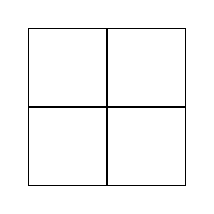
\begin{tikzpicture}
	    \draw (0,0) grid (2,2);
	\end{tikzpicture}
    \end{subfigure}%
    \begin{subfigure}{0.5\textwidth}
	\centering
	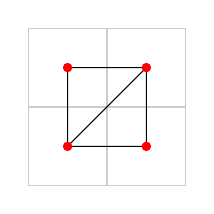
\begin{tikzpicture}
	    \draw[black!20] (0,0) grid (2,2);
	    \draw (0.5,0.5) rectangle (1.5,1.5) -- (0.5,0.5);
	    \filldraw[red] (0.5,0.5) circle [radius=1.5pt]
		      (1.5,0.5) circle [radius=1.5pt]
		      (0.5,1.5) circle [radius=1.5pt]
		      (1.5,1.5) circle [radius=1.5pt];
	\end{tikzpicture}
    \end{subfigure}
    \caption{Gitterwahl für die Diskretisierung: links $2\times 2$ Pixel, rechts zugehöriges Gitter. Die Knotenpunkte liegen in der Mitte der zugehörigen Pixel.}
    \label{fig:grid}
\end{figure}
Für einfache lineare Lagrange Basisfunktionen können die Pixelwerte des Bildes auf diese Weise eins zu eins in der diskreten Funktion als DOF-Vektor repräsentiert werden.
Insbesondere besitzt der entsprechende DOF-Vektor die selbe Anzahl Freiheitsgrade wie das ursprüngliche Bild.

Um Komplikationen zu vermeiden, nutzen alle diskreten Funktionen das selbe Gitter.
In den numerischen Tests wird hierbei das \texttt{alugrid-simplex} Gitter \cite{??} genutzt.
Die diskreten Funktionen sind jedoch teilweise durch unterschiedliche Basisfunktionen repräsentiert.
\begin{itemize}
    \item
	Mit Blick auf die entsprechende partiellen Differentialgleichung \eqref{eq:pde_u} verwenden wir für $u$ lineare Lagrange-Basisfunktionen.
	Für $n$ wären $H^{\mathrm{div}}$-konforme Elemente angebracht (siehe auch \cite{??}).
        Diese standen jedoch in \texttt{dune-fem} nicht zur Verfügung, weshalb gewöhnliche lineare Lagrange-Basisfunktionen für $n$ gewählt wurden.
    \item
	Für $p$ und $m$ wählen wir konstante, diskontinuierliche Basisfunktionen wegen der Ausdrücke $\nabla u$ und $\nabla \cdot n$ im $p$-Update.
	Außerdem sollte sich $m$ auf Grund der Nebenbedingung $|p| - m\cdot p$ im selben diskreten Funktionenraum wie $p$ befinden.
    \item
	Natürlicherweise ergeben sich dann $\lambda_1, \lambda_2$ konstant diskontinuierlich aus den Lagrange-Updates.
    \item
	Unklar ist die Wahl für $\lambda_4$: in jedem Fall wäre eine Projektion nötig, da $n$ und $m$ verschieden repräsentiert sind.
	Wir wählen $\lambda_4$ ebenfalls konstant diskontinuierlich.
\end{itemize}
Diese Wahlen wurden getroffen, um die entstehenden Fehler bei den nötigen Projektionen zwischen verschiedenen diskreten Räumen zu minimieren.
Die nötigen Projektionen befinden sich bei dieser Wahl nur im $m$- und im $\lambda_4$-Update.








\section{Implementierung}


Die Implementierung fand in der Programmiersprache C++ statt.
Verwendet wurden die GPLv2-lizenzierte, C++ „Distributed and Unified Numerics Environment“ Dune\footnote{\url{https://dune-project.org}} samt Core-Modulen, sowie den Modulen \texttt{dune-fem} und \texttt{dune-acfem}.
Dabei ist \texttt{dune-fem} für die Finite Elemente Diskretisierung zuständig und \texttt{dune-acfem} bietet darauf aufbauend eine zusätzliche komfortable Abstraktionsebene.

Ohne die Implementierung im Detail zu beschreiben, soll an dieser Stelle ein kurzer Überblick über die wesentlichen Teile des beiliegenden Quellcodes gegeben werden.
Hinweise zur Installation oder konkreten Verwendung finden sich in der beiliegenden \texttt{README.md}.
Es sei angemerkt, dass Performance nicht das Hauptaugenmerk während der Implementierung darstellte.

\begin{description}
    \item[\texttt{build/src/eeinpaint\{,_gui\}}]
	Die beiden ausführbaren Dateien führen den Inpainting-Algorithmus aus.
 	Das Programm \texttt{build/src/eeinpaint_gui} startet den Algorithmus in einem separaten Thread, um eine in Echtzeit aktualisierte graphische Oberfläche anzuzeigen, auf der die Entwicklung von $u$, sowie verschiedene hilfreiche Werte beobachtet werden können.
	Dagegen ist \texttt{build/src/eeinpaint} rein kommandozeilenbasiert und generiert Log-Daten in Form von Tab-separierten Werten, sowie das Endresultat für $u$ als VTK Unstructured Grid (Endungen \texttt{.pvtu} und \texttt{.vtu}) im Verzeichnis \texttt{output}.

	Parameter können entweder in \texttt{data/parameter} eingestellt werden (siehe unten), oder direkt bei Programmaufruf übergeben werden.
    \item[\texttt{src/algorithm_\{base,live,logging\}.hh}]
	Das Herzstück der Implementierung findet sich in \texttt{algorithm_base.hh}: die Klasse \Code{AlgorithmBase} definiert Methoden für die Teilschritte des Algorithmus, sowie eine Methode \Code{run()}, welche den Algorithmus durchführt.

	Um die Ergebnisse auszugeben, oder zusätzliche Daten während des Algorithmus zu erheben, wird die Klasse durch \Code{AlgorithmLive} und \Code{AlgorithmLogging} entsprechend erweitert.
    \item[\texttt{src/main\{,_gui\}.cc}]
	Dies sind die Programmeinstiegspunkte der beiden generierten ausführbaren Dateien \texttt{src/eeinpaint} und \texttt{src/eeinpaint_gui}.
	Hier wird die Bilddatei für $u^0$ gelesen, das Gitter erzeugt und unter Umständen verfeinert, um anschließend den entsprechenden Algorithmus aufzurufen.
   \item[\texttt{data/input\{,_mask\}.png}]
	Die Datei \texttt{data/input.png} wird in Graustufen gelesen und repräsentiert $u^0$.
	Dazu wird eine Inpainting-Maske aus \texttt{data/input_mask.png} gelesen, welche den Inpaintingbereich angibt: schwarz für $\Omega \setminus D$, weiß für $D$.
    \item[\texttt{data/parameter}]
	Hier werden die nötigen Parameter für den Algorithmus eingestellt.
	Folgende Parameter sind wesentlich.
	\begin{description}
	    \item[\texttt{eeinpaint.\{alpha,beta,eta\}}]
		Parameter $\alpha$, $\beta$, $\gamma$ in der ursprünglichen Inpaintingenergie,
	    \item[\texttt{eeinpaint.\{r1,r2,r4\}}]
		Penaltyparameter für das Augmented Lagrange Verfahren,
	    \item[\texttt{eeinpaint.refinements}]
		Anzahl initialer Verfeinerungen des Gitters,
	    \item[\texttt{eeinpaint.maxOuterIterations}]
		Abbruchkriterium für die Anzahl Schleifendurchläufe in Algorithmus \ref{alg:complete}.
	\end{description}
    \item[\texttt{tools/runjob.sh}]
	Dies ist ein Wrapper für \texttt{build/src/eeinpaint}, um mehrere Jobs parallel laufen lassen zu können.
	Die erzeugten Dateien werden in ein Unterverzeichnis im Ordner \texttt{output} abgelegt, um keine Konflikte zu erzeugen.
    \item[\texttt{tools/vtkconvert.sh}]
	Dieses Skript rendert zweidimensionale VTK Unstructured Grid Dateien mit Endung \texttt{.pvtu} automatisch durch Parallelprojektion zu Graustufen-PNG-Bilder.
\end{description}


Angedacht, aber aus Zeitgründen nicht umgesetzt sind folgende Ideen.
\begin{itemize}
    \item
	Eine adaptive Verfeinerung des Gitters im Laufe des Algorithmus wäre angebracht und könnte die Stärken einer Finiten Elemente Implementierung zum Vorschein bringen.
	Zur Bewertung könnte $|\nabla u|$ dienen, um scharfe Kanten besser auflösen zu können und in weniger interessanten Bereichen des Bildes nicht zu viel Rechenzeit zu verschwenden.
    \item
	Einige Schritte des Algorithmus \ref{alg:complete} sind unabhängig voneinander und könnten parallel arbeiten.
	Abgesehen von den offensichtlich unabhängigen Lagrange-Updates, ist beispielsweise die PDE für $u$ nicht abhängig von $n$ oder $\lambda_4$ im Schritt zuvor, was bedeutet, dass die beiden kostspieligen PDEs parallel berechnet werden könnten.
\end{itemize}

Zu Vergleichszwecken wurde der Algorithmus \ref{alg:complete} in einem separaten Git-Branch auch für reines TV-Inpainting implementiert.
Dabei wurden alle Variablen und Parameter ausgelassen, welche nur für den Krümmungsanteil in der Inpainting-Energie \ref{??} benötigt werden.

\begin{algorithm}[TV Inpainting] \label{alg:tv}
    \Input{$\Omega \subset \R^2$, $u^0: \Omega \setminus D \to \R$, $\alpha, \eta \in \R_{\ge 0}$, $r_2 \in \R_{>0}$} \\
    \Output{$(u^k: \Omega \to \R)_{k\in\N}$}
    \begin{algorithmic}
	\State{$p^0, \lambda_2^0 \gets 0$}
	\For{$k = 0, 1, \dotsc$}
	    \State{$\Big.u^{k+1} \gets \solve{u} 0 = \int_\Omega (r_2 \nabla u - r_2 p^k - \lambda_2^k) \cdot \nabla \phi + \eta \int_{\Omega\setminus D} (u - u^0) \phi$}
	    \State{$\Big.p^{k+1} \gets \max\big\{0, 1 - \frac{\alpha}{q^k}\big\}q^k$, wobei $q^k = \nabla u^k - \frac{\lambda_2^k}{r_2}$}
	    \State{$\Big.\lambda_2^{k+1} \gets \lambda_2^k + r_2(p^k - \nabla u^k)$}
	\EndFor
    \end{algorithmic}
    \begin{note}
	Dieser Algorithmus unterscheidet sich von \ref{alg:complete} mit der Wahl $\beta = 0$, da die Variablen $n, m, \lambda_1, \lambda_4$ nicht mehr auftreten und somit Fehler, die durch Projektionen entstehen, keine Auswirkungen mehr haben.
    \end{note}
\end{algorithm}



\section{Synthetische Tests und Parameterstudie}


Das in den folgenden Tests genutzte, synthetische $u^0$ findet sich in Abbildung \ref{fig:sample}.

\begin{figure}[ht]
    \begin{subfigure}{0.33\textwidth}
	\centering
	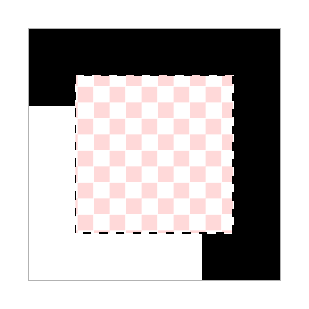
\begin{tikzpicture}[scale=0.1]
	    \filldraw[black] (0,0) rectangle (32,32);
	    \filldraw[white] (0,0) rectangle (22,22);
	    \filldraw[white] (6,6) rectangle (26,26);
	    \draw[missing] (6,6) rectangle (26,26);
	    \draw[black!30] (0,0) rectangle (32,32);
	\end{tikzpicture}
    \end{subfigure}%
    \begin{subfigure}{0.33\textwidth}
	\centering
	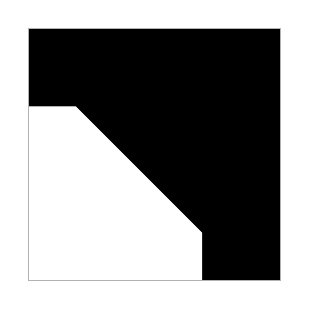
\begin{tikzpicture}[scale=0.1]
	    \filldraw[black] (0,0) rectangle (32,32);
	    \filldraw[white] (0,0) -- (22,0) -- (22,6) -- (6,22) -- (0,22) -- cycle;
	    \draw[black!30] (0,0) rectangle (32,32);
	\end{tikzpicture}
    \end{subfigure}%
    \begin{subfigure}{0.33\textwidth}
	\centering
	
\begin{tikzpicture}[scale=0.1]
	    \clip (0,0) rectangle (32,32);
	    \filldraw[black] (0,0) rectangle (32,32);
	    \filldraw[white,rounded corners=50] (-22,-22) rectangle (22,22);
	    \draw[black!30] (0,0) rectangle (32,32);
	\end{tikzpicture}
    \end{subfigure}%
    \caption{In den numerischen Tests vorgegebenes $32\times 32$ Pixel Inpaintingproblem (links) zusammen mit theoretisch wünschenswertem TV-Inpainting (mittig) und Elastica-Inpainting (rechts)}
    \label{fig:sample}
\end{figure}

Für TV-Inpainting erwarten wir als Lösung eine diagonale, gerade verlaufende Schwarz-Weiß-Kante, während Elastica-Inpainting eine (je nach Wahl von $\alpha, \beta$) gekrümmte Kante hervorbringen sollte.

\DeclareDocumentCommand{\kmax}{}{k_{\mathrm{max}}}
Zwei Abbruchkriterien wurden implementiert:
\begin{itemize}
    \item
	Eine maximale Anzahl Iterationen wurde erreicht:
	\begin{math}[numbered] \label{eq:stopmax}
	    k > \kmax.
	\end{math}
    \item
	Die Summe der Residuen in den Lagrange-Updates der Nebenbedingungen ist hinreichend klein:
	\begin{math}[numbered] \label{eq:stopres}
	    \underbrace{\||p^k| - m^k \cdot p^k\|_{L^2}}_{=:R_{mp}^k} + \underbrace{\|p^k - \nabla u^k\|_{L^2}}_{=:R_{pu}^k} + \underbrace{\|n^k - m^k\|_{L^2}}_{=:R_{nm}^k} < \epsilon_R.
	\end{math}
\end{itemize}

\DeclareDocumentCommand{\Limg}{}{\scr L_{\mathrm{img}}}
\DeclareDocumentCommand{\Ldat}{}{\scr L_{\mathrm{dat}}}
\DeclareDocumentCommand{\Lconstr}{}{\scr L_{\mathrm{constr}}}
\DeclareDocumentCommand{\Ltotal}{}{\scr L_{\mathrm{total}}}

Wir protokollieren unter anderem
die $L^2$-Abstände aufeinanderfolgender Itererierten, obige Lagrange-Update Residuen $R_{mp}^k$, $R_{pu}^k$, $R_{nm}^k$, sowie
die numerischen Energien
\begin{math}
    \Limg^k &:= \int_\Omega \big(\alpha + \beta (\nabla \cdot n^k)^2\big)|p^k|, \\
    \Ldat^k &:= \frac{\eta}{2} \int_{\Omega\setminus D} |u^k - u^0|^2, \\
    \Lconstr^k &:=
	r_1 \int_\Omega (|p^k| - m^k\cdot p^k) + \int_\Omega \lambda_1 (|p^k| - m^k \cdot p^k) \\
	&\quad + \frac{r_2}{2} \int_\Omega |p^k - \nabla u^k|^2 + \int_\Omega \lambda_2 \cdot (p^k - \nabla u^k) \\
	&\quad + \frac{r_4}{2} \int_\Omega |n^k - m^k|^2 + \int_\Omega \lambda_4 \cdot (n^k - m^k), \\
    \Ltotal^k &:= \Limg^k + \Ldat^k + \Lconstr^k.
\end{math}

In den Tests zur Gitterverfeinerung bezeichnen wir mit $q \in \N$ die Anzahl globaler Verfeinerungen.
Bei dem hier genutzten Gitter bedeutet eine globale Verfeinerung die Bisektion jedes Dreiecks.



%\begin{math}
%    \|u^k - u^{k-1}\|,
%    \|p^k - p^{k-1}\|,
%    \|m^k - m^{k-1}\|,
%    \|n^k - n^{k-1}\|,
%    \|\lambda_1^k - \lambda_1^{k-1}\|,
%    \|\lambda_2^k - \lambda_2^{k-1}\|,
%    \|\lambda_4^k - \lambda_4^{k-1}\|.
%\end{math}

\subsection*{TV-Inpainting}

Wir testen nun den TV-Inpainting-Algorithmus \ref{alg:tv} und führen eine kleine Parameterstudie für $r_2$ durch.
Hierfür wählen wir $\alpha = 1$ und $\eta = 1000$, während wir $r_2 \in \Set{10^k}_{k=-2}^4$ variieren.
Als Abbruchkriterium wurde \eqref{eq:stopmax} mit $\kmax = 5000$ gewählt.

\DeclareDocumentCommand{\Etv}{}{E_{\mathrm{tv}}}

Die Inpainting-Energie aus \eqref{eq:energy_ee} ist hier von der Form
\begin{math}
    \Etv = \int_\Omega \alpha |\nabla u| + \frac{\eta}{2} \int_{\Omega\setminus D} |u - u^0|^2.
\end{math}
Da wir für $u$ lineare Basisfunktionen angesetzt haben, lässt sich $E_{\mathrm{tv}}[u]$ ohne weiteres numerisch auswerten.
\begin{figure}[ht]
    \centering
    \begin{tikzpicture}
	\begin{semilogxaxis}[width=10cm,height=6cm,xlabel=$k$,ylabel={$E_{\mathrm{tv}}[u^k]$},restrict y to domain=260:268]
	    %\addplot table [x=k,y=dataEnergy] {refinements=0_alpha=1e0_r2=1e-2/output.dat};
	    %\addplot table [x=k,y=tv] {refinements=0_alpha=1e0_r2=1e-2/output.dat};
	    \addplot table [x=k,y expr=\thisrow{tv}+\thisrow{dataEnergy}] {data/tvr2/refinements=0_alpha=1e0_r2=1e-2/output.dat};
	    \addplot table [x=k,y expr=\thisrow{tv}+\thisrow{dataEnergy}] {data/tvr2/refinements=0_alpha=1e0_r2=1e-1/output.dat};
	    \addplot table [x=k,y expr=\thisrow{tv}+\thisrow{dataEnergy}] {data/tvr2/refinements=0_alpha=1e0_r2=1e0/output.dat};
	    \addplot table [x=k,y expr=\thisrow{tv}+\thisrow{dataEnergy}] {data/tvr2/refinements=0_alpha=1e0_r2=1e1/output.dat};
	    \addplot table [x=k,y expr=\thisrow{tv}+\thisrow{dataEnergy}] {data/tvr2/refinements=0_alpha=1e0_r2=1e2/output.dat};
	    \addplot table [x=k,y expr=\thisrow{tv}+\thisrow{dataEnergy}] {data/tvr2/refinements=0_alpha=1e0_r2=1e3/output.dat};
	    \addplot table [x=k,y expr=\thisrow{tv}+\thisrow{dataEnergy}] {data/tvr2/refinements=0_alpha=1e0_r2=1e4/output.dat};
	    \legend{
	      $r_2=10^{-2}$,
	      $r_2=10^{-1}$,
	      $r_2=10^0$,
	      $r_2=10^1$,
	      $r_2=10^2$,
	      $r_2=10^3$,
	      $r_2=10^4$,
	    }
	\end{semilogxaxis}
    \end{tikzpicture}
    \caption{TV-Inpainting-Energie für verschiedene Penaltyparameter.}
    \label{fig:num_tvr2_etv}
\end{figure}
In Abbildung \ref{fig:num_tvr2_etv} sehen wir, dass die Energie $\Etv$ für alle Parameterwahlen $r_2$ annähernd gegen den selben Wert konvergiert.
Das beste Konvergenzverhalten ist für $r_2 = 10$ zu beobachten.
Im Endergebnis für $k = 5000$ unterscheidet sich nur der Fall $r_2 = 10^4$ mit der höchsten Energie noch optisch von den restlichen Ergebnissen, wie exemplarisch in Abbildung \ref{fig:num_tvr2_png} zu sehen.

\begin{figure}[ht]
    \centering
    \begin{subfigure}{0.2\textwidth}
	\centering
	\myincludegraphics[width=0.8\textwidth]{data/tvr2/refinements=0_alpha=1e0_r2=1e-2/vtk.png}
	\caption{$r_2=10^{-2}$}
    \end{subfigure}%
    \begin{subfigure}{0.2\textwidth}
	\centering
	\myincludegraphics[width=0.8\textwidth]{data/tvr2/refinements=0_alpha=1e0_r2=1e2/vtk.png}
	\caption{$r_2=10^{1}$}
    \end{subfigure}%
    \begin{subfigure}{0.2\textwidth}
	\centering
	\myincludegraphics[width=0.8\textwidth]{data/tvr2/refinements=0_alpha=1e0_r2=1e4/vtk.png}
	\caption{$r_2=10^{4}$}
    \end{subfigure}%
    \caption{Inpaintingresultate für verschiedene $r_2$}
    \label{fig:num_tvr2_png}
\end{figure}

Für $r_2 \ge 10$ wird die Nebenbedingung $p = \nabla u$ durchgehend besser eingehalten (siehe Abbildung \ref{num_tvr2_pu}) auf Kosten einer zu Beginn sehr hohen Energie $\Etv$.
Für $r_2 \le 1$ ist die Energie zu Beginn relativ niedrig, erfährt jedoch erst einen deutlichen Abfall nachdem die Nebenbedingungen zu einem gewissen Grad eingehalten wurden.

\begin{figure}[ht]
    \centering
    \begin{tikzpicture}
	\begin{loglogaxis}[width=10cm,xlabel=$k$,ylabel={$R_{pu}$}]
	    %\addplot table [x=k,y=dataEnergy] {refinements=0_alpha=1e0_r2=1e-2/output.dat};
	    %\addplot table [x=k,y=tv] {refinements=0_alpha=1e0_r2=1e-2/output.dat};
	    \addplot table [x=k,y=puConstr] {data/tvr2/refinements=0_alpha=1e0_r2=1e-2/output.dat};
	    \addplot table [x=k,y=puConstr] {data/tvr2/refinements=0_alpha=1e0_r2=1e-1/output.dat};
	    \addplot table [x=k,y=puConstr] {data/tvr2/refinements=0_alpha=1e0_r2=1e0/output.dat};
	    \addplot table [x=k,y=puConstr] {data/tvr2/refinements=0_alpha=1e0_r2=1e1/output.dat};
	    \addplot table [x=k,y=puConstr] {data/tvr2/refinements=0_alpha=1e0_r2=1e2/output.dat};
	    \addplot table [x=k,y=puConstr] {data/tvr2/refinements=0_alpha=1e0_r2=1e3/output.dat};
	    \addplot table [x=k,y=puConstr] {data/tvr2/refinements=0_alpha=1e0_r2=1e4/output.dat};
	    \legend{
	      $r_2=10^{-2}$,
	      $r_2=10^{-1}$,
	      $r_2=10^0$,
	      $r_2=10^1$,
	      $r_2=10^2$,
	      $r_2=10^3$,
	      $r_2=10^4$,
	    }
	\end{loglogaxis}
    \end{tikzpicture}
    \caption{Residuum $\|p - \nabla u\|_{L^2}$ für verschiedene Penaltyparameter.}
    \label{fig:num_tvr2_pu}
\end{figure}


% TODO: echte tv energie, vs numerische mit p



Anzumerken ist in Abbildung \ref{fig:num_tvr2_png} die Verwaschenheit der diagonalen Kante, sowie die beiden kleinen Auswüchse an den jeweiligen Enden dieser.
Beides reduziert sich durch globale Verfeinerung des Gitters, wie in Abbildung \ref{fig:num_tvrefine_png} zu sehen.

\begin{figure}[ht]
    \centering
    \begin{subfigure}{0.2\textwidth}
	\centering
	\myincludegraphics[width=0.8\textwidth]{data/tvrefine/refinements=0_alpha=1e0_r2=1e1/vtk.png}
	\caption{$q=0$}
    \end{subfigure}%
    \begin{subfigure}{0.2\textwidth}
	\centering
	\myincludegraphics[width=0.8\textwidth]{data/tvrefine/refinements=1_alpha=1e0_r2=1e1/vtk.png}
	\caption{$q=1$}
    \end{subfigure}%
    \begin{subfigure}{0.2\textwidth}
	\centering
	\myincludegraphics[width=0.8\textwidth]{data/tvrefine/refinements=4_alpha=1e0_r2=1e1/vtk.png}
	\caption{$q=4$}
    \end{subfigure}%
    \caption{Verfeinerung des Gitters für $r_2=10^1$.}
    \label{fig:num_tvrefine_png}
\end{figure}

%\begin{figure}[ht]
%    \centering
%    \begin{tikzpicture}
%	\begin{semilogxaxis}[width=10cm,height=6cm,xlabel=$k$,ylabel={$E_{\mathrm{tv}}[u^k]$}]
%	    %\addplot table [x=k,y=dataEnergy] {refinements=0_alpha=1e0_r2=1e-2/output.dat};
%	    %\addplot table [x=k,y=tv] {refinements=0_alpha=1e0_r2=1e-2/output.dat};
%	    \addplot table [x=k,y expr=\thisrow{tv}] {data/tvrefine/refinements=0_alpha=1e0_r2=1e1/output.dat};
%	    \addplot table [x=k,y expr=\thisrow{tv}] {data/tvrefine/refinements=1_alpha=1e0_r2=1e1/output.dat};
%	    \addplot table [x=k,y expr=\thisrow{tv}] {data/tvrefine/refinements=2_alpha=1e0_r2=1e1/output.dat};
%	    \addplot table [x=k,y expr=\thisrow{tv}] {data/tvrefine/refinements=3_alpha=1e0_r2=1e1/output.dat};
%	    \addplot table [x=k,y expr=\thisrow{tv}] {data/tvrefine/refinements=4_alpha=1e0_r2=1e1/output.dat};
%	    \legend{
%	      $q=0$,
%	      $q=1$,
%	      $q=2$,
%	      $q=3$,
%	      $q=4$,
%	    }
%	\end{semilogxaxis}
%    \end{tikzpicture}
%    \caption{Totale Variation bei unterschiedlicher globaler Verfeinerung.}
%    \label{fig:num_tvrefine_tv}
%\end{figure}


\subsection*{Euler Elastica Inpainting}

Wenden wir uns nun Algorithmus \ref{alg:ee} zu.
Auch hier wünschen wir uns numerisch eine Konvergenz des Algorithmus und möglichst von den Penaltyparametern $r_1, r_2, r_4$ unabhängige Endresultate.
Wir fixieren zunächst $\eta = 1000$ und untersucht dies mit zwei Parameterstudien.

Wir fixieren zunächst $\alpha = 1$ und $\beta = 1000$ und variieren
\begin{math}[numbered] \label{eq:num_param}
    r_1 \in \Set{10^0, 10^1, 10^2, 10^3, 10^4}, \qquad
    r_2 \in \Set{10^0, 10^2, 10^4}, \qquad
    r_4 \in \Set{10^0, 10^2, 10^4}.
\end{math}
Für $r_1$ wurde eine feinere Auflösung gewählt, da die Modifikation in \eqref{eq:energy_al} (die Verwendung von $L^1$-Penalizing statt $L^2$-Penalizing) höchstwahrscheinlich starke Auswirkungen auf die Größenordnung von $r_1$ hat.
Als Abbruchkriterium wird an dieser Stelle \eqref{eq:stopmax} gewählt mit $\kmax = 50000$.


Für hohe Parameter $r_2, r_4$ und niedriges $r_1$ zeigt der Algorithmus ein konvergentes Verhalten (siehe \ref{fig:num_eeparam_conv} und man beobachtet Ergebnisse wie in \ref{fig:num_eeparam_png}.
Diese Bilder zeigen die für das Elastica-Inpainting erwünschte gekrümmte Kante.
Leider scheint das Inpaintingresultat vom Parameter $r_1$ abzuhängen und man beobachtet in \ref{fig:num_eeparam_png} für höheres $r_1$ eine stärker nach außen gebogene Kante.



\begin{figure}[ht]
    \centering
    \begin{tikzpicture}
	\begin{loglogaxis}[width=10cm,height=6cm,xlabel=$k$,ylabel={$\|u_k - u_{k-1}\|_{L^2}$}]
	    \addplot table [x=k,y=uDist] {data/eeparam/refinements=0_alpha=1e0_beta=1e3_r1=1e0_r2=1e4_r4=1e4/output.dat};
	    \addplot table [x=k,y=uDist] {data/eeparam/refinements=0_alpha=1e0_beta=1e3_r1=1e1_r2=1e4_r4=1e4/output.dat};
	    \addplot table [x=k,y=uDist] {data/eeparam/refinements=0_alpha=1e0_beta=1e3_r1=1e2_r2=1e4_r4=1e4/output.dat};
	    \legend{
	      $r_1 = 1$,
	      $r_1 = 10$,
	      $r_1 = 100$,
	    }
	\end{loglogaxis}
    \end{tikzpicture}
    \caption{$\|u_k - u_{k-1}\|_{L^2}$ für $r_1 \ll r_2, r_4$.}
    \label{fig:num_eeparam_conv}
\end{figure}



\begin{figure}[ht]
    \centering
    \begin{subfigure}{0.2\textwidth}
	\centering
	\myincludegraphics[width=0.8\textwidth]{data/eeparam/refinements=0_alpha=1e0_beta=1e3_r1=1e0_r2=1e4_r4=1e4/vtk.png}
	\caption{$r_1 = 1$}
    \end{subfigure}%
    \begin{subfigure}{0.2\textwidth}
	\centering
	\myincludegraphics[width=0.8\textwidth]{data/eeparam/refinements=0_alpha=1e0_beta=1e3_r1=1e1_r2=1e4_r4=1e4/vtk.png}
	\caption{$r_1 = 10$}
    \end{subfigure}%
    \begin{subfigure}{0.2\textwidth}
	\centering
	\myincludegraphics[width=0.8\textwidth]{data/eeparam/refinements=0_alpha=1e0_beta=1e3_r1=1e2_r2=1e4_r4=1e4/vtk.png}
	\caption{$r_1 = 100$}
    \end{subfigure}%
    \caption{$\|u_k - u_{k-1}\|_{L^2}$ für $r_1 \ll r_2, r_4 = 10^4$.}
    \label{fig:num_eeparam_png}
\end{figure}











\section{Praktische Anwendungen und Beobachtungen}

%\begin{itemize}
%    \item
%	Gitterwahl: structured (simplex/kubisch) oder unstructured (simplex, guiding durch Kantendetektor)
%    \item
%	Lineare Lagrange Basis-Funktionen als nahezu einzige Wahl
%    \item
%	Adaptive Strategien (z.B. refine/coarse gemäß $n = \nabla u$), Vergleich
%    \item
%	Parameter-Tweaking ($\alpha$, $\beta$, $\eta$, $r_1, r_2, r_3, r_4$) und -Interpretation
%    \item
%	Startwert-Tweaking ($v, u, m, p, n, \lambda_1, \lambda_2, \lambda_3, \lambda_4$)
%\end{itemize}


\bibliographystyle{plain}
\bibliography{thesis}

\end{document}

